% !TEX root = Tesi.tex
\chead{}

\chapter{Enhancing web models via model transformations}
\label{enhancing-web-models-via-model-transformations}

\section{Transformation}

In the last chapter, after describing both metamodels for the Real Usage Data and the Interaction Flow Modeling Language,  we proceeded to create dynamic instances for both models respectively describing the actual input data available for the personalization process and the initial IFMLModel of the eCommerce Madison Island website. In this chapter, we illustrate a possible model transformation for this model based on the Real Usage instance data with the goal of creating an upgraded model version which takes into account the customer preferences and his actions.

\subsection{Homepage updates}
\label{homepage-updates}
Considering the data coming from the Proximity sensors within the actual Madison Island retail store we are aware of a set of regions corresponding to the categories the user prefers over the others, this information will be used to change the content, and therefore the IFMLModel, for the Homepage carousel.

For instance, we know that \textbf{Blazers},\textbf{Tees, Knits and Polos} and \textbf{Shoes} categories correspond to the \textit{sessionRegion} elements where the user spent more time within the store after sorting the entries by \textit{maxSecondsInRegion} and \textit{maxProximity}. In the case of the Blazers category for example, the data belonging to the \textit{RealUsageData:ProximityData} parent node has this form:

\vspace{0.5cm}
\lstset{language=XML}
\begin{lstlisting} 
  <sessionRegions
  regionId="40"
  regionLabel="blazers"
  detectionCount="1"
  maxSecondsInRegion="195"
  maxProximity="immediate"
  firstDetectionTimeStamp="2018-02-21T18:11:01.000+0100"
  lastDetectionTimeStamp="2018-02-21T18:11:01.000+0100">
  <beaconData
    uuid="0686a88e-fed6-11e7-8be5-0ed5f89f718b"
    majorId="25911"
    minorId="27"/>
</sessionRegions>
\end{lstlisting}
\vspace{0.5cm}

Applying this knowledge, the \textit{subBiewComponentParts} and the \textit{parameter} nodes of the first HightlightedCategoriesCarousel \textit{IFMLWindow} elements from the initial \textit{IFMLModel} can be modified from this:

\vspace{0.5cm}
\lstset{language=XML}
\begin{lstlisting} 
<parameters  name="Highlighted Category #1" direction="inout">
  <constraints  language="SQL" body="Category.ID=18"/>
</parameters>

...

<subViewComponentParts xsi:type="core:ConditionalExpression"  language="SQL" body="Category.ID=18" name="Eyewear"/>
\end{lstlisting}
\vspace{0.5cm}

to :

\vspace{0.5cm}
\lstset{language=XML}
\begin{lstlisting} 
  <parameters  name="Highlighted Category #1" direction="inout">
  <constraints  language="SQL" body="Category.ID=40"/>
</parameters>

...

<subViewComponentParts xsi:type="core:ConditionalExpression"  language="SQL" body="Category.ID=40" name="Blazers"/>
\end{lstlisting}
\vspace{0.5cm}

Besides this content update which priorities some categories over the others, the \textit{IFMLModel} can also be transformed to use different IFML elements under certain conditions. For example, the viewComponent which is responsible for displaying the most recent products on the homepage can be swapped with another \textit{List View Component} responsible for presenting the latest products the customer interacted with in the physical retail store. The information about these products is available in the RealUsageData model under the \textit{RealUsageData:ActionData} section and, in our specific example, it carries the data about the product SKUs the customer scanned with his smartphone camera to collect reward points.

\vspace{0.5cm}
\lstset{language=XML}
\begin{lstlisting} 
<sessionActions userAgent="iPhone 6S">
  <scannedItems 
  barcode="042100005264" name="Elizabeth Knit Top-Red-S" sku="wbk012c-Red-S"/>
  <scannedItems 
  barcode="042100005931" name="Plaid Cotton Shirt-Khaki-L" sku="msj006c-Khaki-L"/>
  <scannedItems 
  barcode="042100007717" name="Broad St Saddle Shoes" sku="shm00110"/>
</sessionActions>
\end{lstlisting}
\vspace{0.5cm}


The model transition in this case would occurr not only replacing the IFML viewComponent with a different type but also adding a \textit{ConditionalExpression} filtering the items by their SKUs as per shown in Figure \ref{fig:ifml-transformation-example}.

\vspace{0.5cm}
\begin{figure}[H]
  \centering
    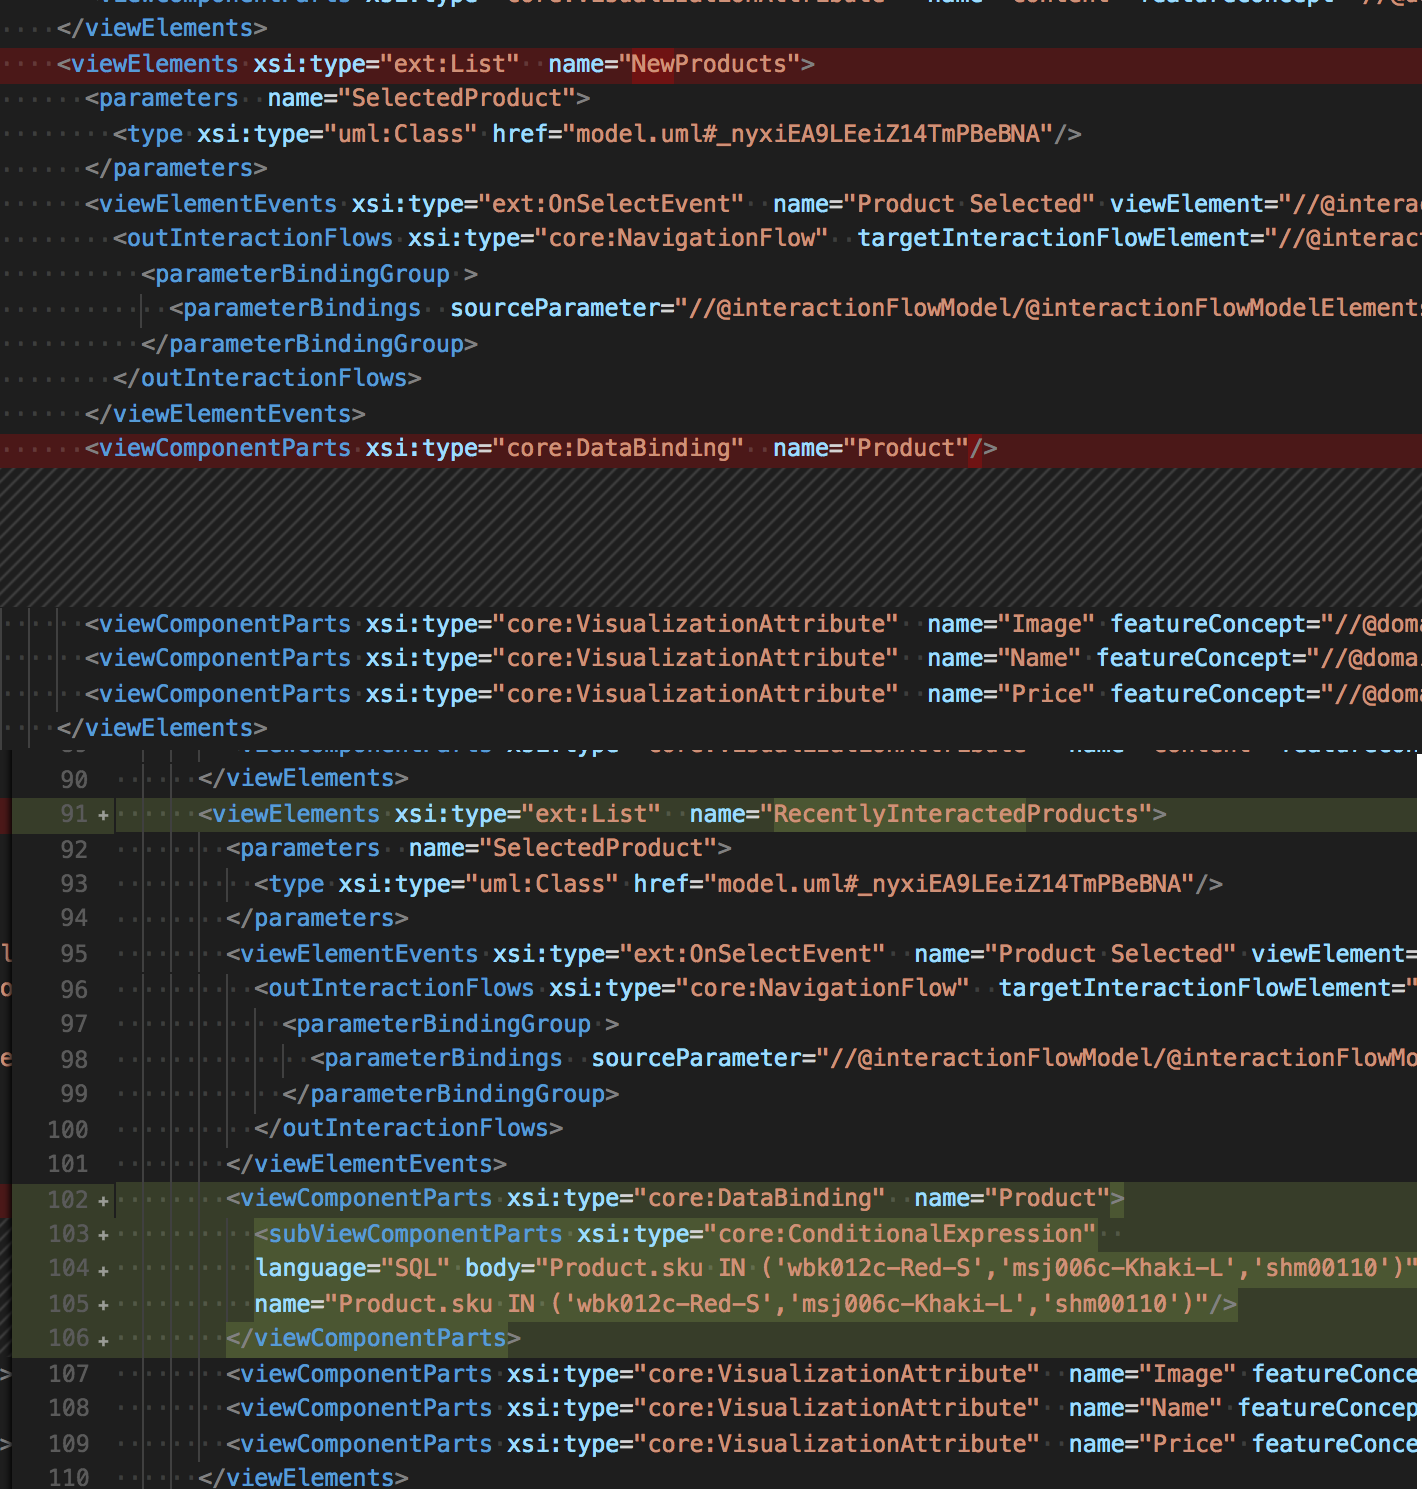
\includegraphics[height=12cm]{images/madison/ifm-homepage-transformation.png}
  \caption{IFML Homepage transformation example}
  \label{fig:ifml-transformation-example}
\end{figure}
\vspace{0.5cm}

\subsection{Header updates}
\label{header-updates}
Leveraging once more the \textit{RealUsageData:ActionData}, the Header node of the IFMLModel describing the Madison Island website top area could also be enhanced to show a list of recent actions which generated reward points performed by the customer in the physical stores.  This is achieved appending  an instance of \textit{List View Component} to the \textit{interactionFlowModelElements} parent node called \textit{RecentRewardActions} linked to the Rewards \textit{Data Binding} entity and visualizing the \textit{Action Name} and \textit{Points Attribution} properties to the frontend as per shown in the following snippet of code of the \textit{IFMLModel}:

\vspace{0.5cm}
\lstset{language=XML}
\begin{lstlisting} 
  <interactionFlowModelElements xsi:type="ext:IFMLWindow"  name="Header" isLandmark="true">
  <viewElements xsi:type="ext:List"  name="NavigationMenu">
   ...
  </viewElements>
  <viewElements xsi:type="ext:Form"  name="SearchForm">
   ...
  </viewElements>
  <viewElements xsi:type="core:ViewComponent"  name="TopLinks"/>
  <viewElements xsi:type="core:ViewComponent"  name="LanguageSwitch"/>

  <!-- ADDED NODE -->
  <viewElements xsi:type="ext:List"  name="RecentRewardActions">
    <viewComponentParts xsi:type="core:DataBinding"  name="Rewards" domainConcept="//@domainModel/@domainElements.13"/>
    <viewComponentParts xsi:type="core:VisualizationAttribute"  name="Action Name" featureConcept="//@domainModel/@domainElements.15"/>
    <viewComponentParts xsi:type="core:VisualizationAttribute"  name="Points Attribution" featureConcept="//@domainModel/@domainElements.14"/>
  </viewElements>
  <!-- ADDED NODE -->

  </interactionFlowModelElements>
\end{lstlisting}
\vspace{0.5cm}

\subsection{Category Page Updates}
\label{category-page-updates}
In light of the information gathered in the Real Usage Data model about the recently viewed products available in the \textit{RealUsageData:WebData} node, the Category page can be enhanced appending an additional visual element to the user interface to track this information.

To do so, we filter out the RealUsageData model fetching the nodes containing a \textit{parameterBindingGroup} property including a Product reference like the following entries :

\vspace{0.5cm}
\lstset{language=XML}
\begin{lstlisting} 
      <data xsi:type="RealUsageData:WebData"
      ID="3"
      name="AccessLog"
      userID="3045678"
      date="2017-11-29T07:08:40.000+0100"
      viewContainer="Category #15"
      viewComponent="ProductList"
      eventType="click"
      parameterBindingGroup="Product/404"
      logEntry="GET /men/shirts/plaid-cotton-shirt-476.html 200 0 - 29505"/>
      
      <data xsi:type="RealUsageData:WebData"
      ID="4"
      name="AccessLog"
      userID="3045678"
      date="2017-12-04T06:37:15.000+0100"
      viewContainer="Product #404"
      viewComponent="RelatedProductList"
      eventType="click"
      parameterBindingGroup="Product/413"
      logEntry="GET /core-striped-sport-shirt-551.html 200 0 - 29505"/>

      <data xsi:type="RealUsageData:WebData"
      ID="8"
      name="AccessLog"
      userID="3045678"
      date="2017-12-04T06:38:20.000+0100"
      viewContainer="Search Results"
      viewComponent="ProductList"
      eventType="click"
      parameterBindingGroup="Product/407"
      logEntry="GET /stretch-cotton-blazer-587.html 200 0 - 29505"/>
\end{lstlisting}
\vspace{0.5cm}

With the above data we can then proceed transforming the intial IFML Model for the Category page appending a \textit{RecentlyViewedProducts} section in the form of a \textit{List View Component} bound to the Product \textit{Data Binding} entity.

This new IFML item would be responsible for presenting the thumbnails, names and prices of these products to the customer separating them through a distinct \textit{ConditionalExpression} which maps the children node of the \textit{RealUsageData:WebData} dataset shown earlier before finally returning the items in the order they were browsed regardless of the display mode property of the Category itself (Figure \ref{fig:recently-viewed-ifml-definition}).

\vspace{0.5cm}
\begin{figure}[H]
  \centering
    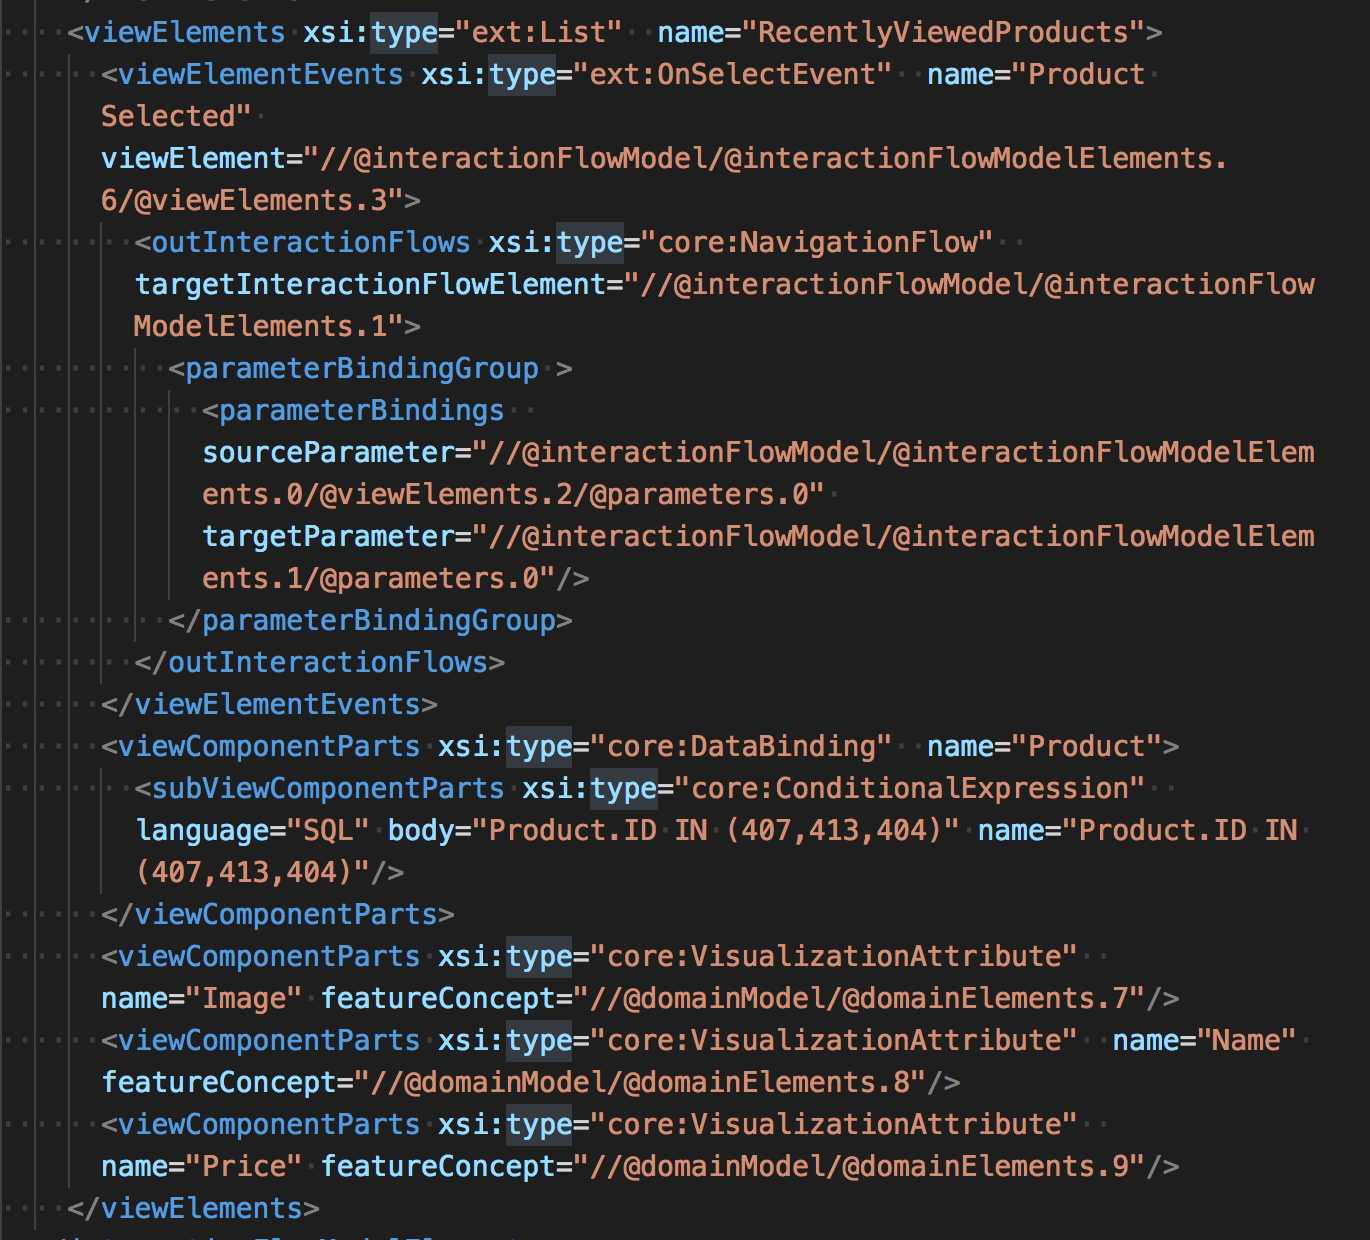
\includegraphics[height=12cm]{images/madison/ifml-recently-viewed.png}
  \caption{Recently Viewed IFML definition snippet}
  \label{fig:recently-viewed-ifml-definition}
\end{figure}
\vspace{0.5cm}

\subsection{Product Page Updates}
\label{product-page-updates}

For what it involves the possible improvements on the product page of the Madison Island website, we concentrated on the Related Products widget shown just below the Add To Cart section. In the first \textit{IFMLModel} the list of the products related to the currently shown one has no particular logic assigned, our potential transformation can extend the \textit{viewElements} node of the \textit{IFMLModel} taking into consideration the browsing pattern of the users which have been identified examining the RealUsageData instances entries.

For example, we could have discovered that the \textbf{Core Striped Sport Shirt} product page is frequently browsed along with the \textbf{Plaid Cotton Shirt} product page during the same recorded sessions analyzing the values set in the \textit{viewContainer}, \textit{viewComponent} and \textit{parameterBindingGroup} properties for the nodes belonging to the \textit{RealUsageData:WebData} dataset. Due to this, we can take advantage of this correlation to push a product rather than another on the Related Products section for those products consequently offering a more tailored and customized experience to the user.

The transformation on the starting \textit{IFMLModel} that would occur in this case restricts the \textit{Data Binding} scope appending a \textit{subViewComponentParts} to it which limits the products collection to the computed set of related products SKUs. This additional \textit{ConditionalExpression} would also be bound to a specific \textit{ActivationExpression} which would enable the above filtering only when a customized collection for the current product is available. 

From a \textit{IFMLModel} code perspective, for the \textit{List View Component} which controls the Related Product widget we would transition from this node configuration :

\vspace{0.5cm}
\lstset{language=XML}
\begin{lstlisting} 
  <viewElements xsi:type="ext:List"  name="RelatedProductList">
  <viewElementEvents xsi:type="ext:OnSelectEvent"  name="Product Selected" viewElement="//@interactionFlowModel/@interactionFlowModelElements.1/@viewElements.2">
    ...
  </viewElementEvents>
  <viewComponentParts xsi:type="core:DataBinding"  name="Product"/>
  <viewComponentParts xsi:type="core:VisualizationAttribute"  name="Image" featureConcept="//@domainModel/@domainElements.7"/>
  <viewComponentParts xsi:type="core:VisualizationAttribute"  name="Name" featureConcept="//@domainModel/@domainElements.8"/>
  <viewComponentParts xsi:type="core:VisualizationAttribute"  name="Price" featureConcept="//@domainModel/@domainElements.9"/>
</viewElements>
\end{lstlisting}
\vspace{0.5cm}

to this one :

\vspace{0.5cm}
\lstset{language=XML}
\begin{lstlisting} 
  <viewElements xsi:type="ext:List"  name="RelatedProductList">
  <viewElementEvents xsi:type="ext:OnSelectEvent"  name="Product Selected" viewElement="//@interactionFlowModel/@interactionFlowModelElements.1/@viewElements.2">
      ...
  </viewElementEvents>
  <viewComponentParts xsi:type="core:DataBinding"  name="Product">
    <subViewComponentParts xsi:type="core:ConditionalExpression"  language="SQL" body="Product.ID IN getCustomizedRelatedProducts()" name="Product.ID IN getCustomizedRelatedProducts" activationExpression="//@interactionFlowModel/@interactionFlowModelElements.17"/>
  </viewComponentParts>
  <viewComponentParts xsi:type="core:VisualizationAttribute"  name="Image" featureConcept="//@domainModel/@domainElements.7"/>
  <viewComponentParts xsi:type="core:VisualizationAttribute"  name="Name" featureConcept="//@domainModel/@domainElements.8"/>
  <viewComponentParts xsi:type="core:VisualizationAttribute"  name="Price" featureConcept="//@domainModel/@domainElements.9"/>
</viewElements>
\end{lstlisting}
\vspace{0.5cm}

Moreover, the \textit{ActivationExpression} defined by the \textit{interactionFlowModelElements} XPath expression presented in the above snippet  links to a node responsible for the control of the feature with the following content:

\vspace{0.5cm}
\lstset{language=XML}
\begin{lstlisting} 
<interactionFlowModelElements 
  xsi:type="core:ActivationExpression" id="CurrentProduct.hasCustomizedRelatedProduct" language="SQL" body="CurrentProduct.hasCustomizedRelatedProduct()">
</interactionFlowModelElements>

\end{lstlisting}
\vspace{0.5cm}
\subsection{Shopping Cart updates}

As per described in \ref{shopping-cart-page-overview}, the Shopping Cart page model includes two main sections: a \textit{List Product List} component responsible for the interactions with the cart items and a \textit{IFMLWindow} for grouping the actions the customer may trigger through the interface for applying discounts or estimating shipping and taxes on his current quote.

As for the previous cases, applying the data from the Real Data Usage model, we can modify and extend the interaction flow of this page adding a brand new \textit{View Component} responsible for showing the Reward points the user accumulated within the Shopping Cart Sidebar. The component not only displays the information by the  \textit{Data Binding} with the Reward entity but it also controls the \textit{Event} associated with the \textbf{"Apply Discount"} button and the \textit{Action} connected to it.

\section{Updated web models}

%\addcontentsline{toc}{chapter}{}

\subsubsection{Homepage overview}

The Madison Island Interaction Model for the Homepage (Figure \ref{fig:desktop-before-homepage} and \ref{fig:ifml-before-homepage}) is composed by a parent \textit{IFMLWindow} element which contains three children elements: respectively another \textit{IFMLWindow} for the Highlighted Categories Carousel, a \textit{Detail View Component} for the Homepage promos CMS Block and a \textit{List View Component} for the New Products sections bound to the Product Entity of the domain model. The HighlightedCategoriesCarousel Window is in \textit{XOR mode} representing three possible scenarios for the category to promote with the highest priority within the carousel mechanism. Each data binding within all these view containers is limited by a \textit{Conditional Expressions} defining the instance of the content to show.

\vspace{0.5cm}
\begin{figure}[H]
  \centering
    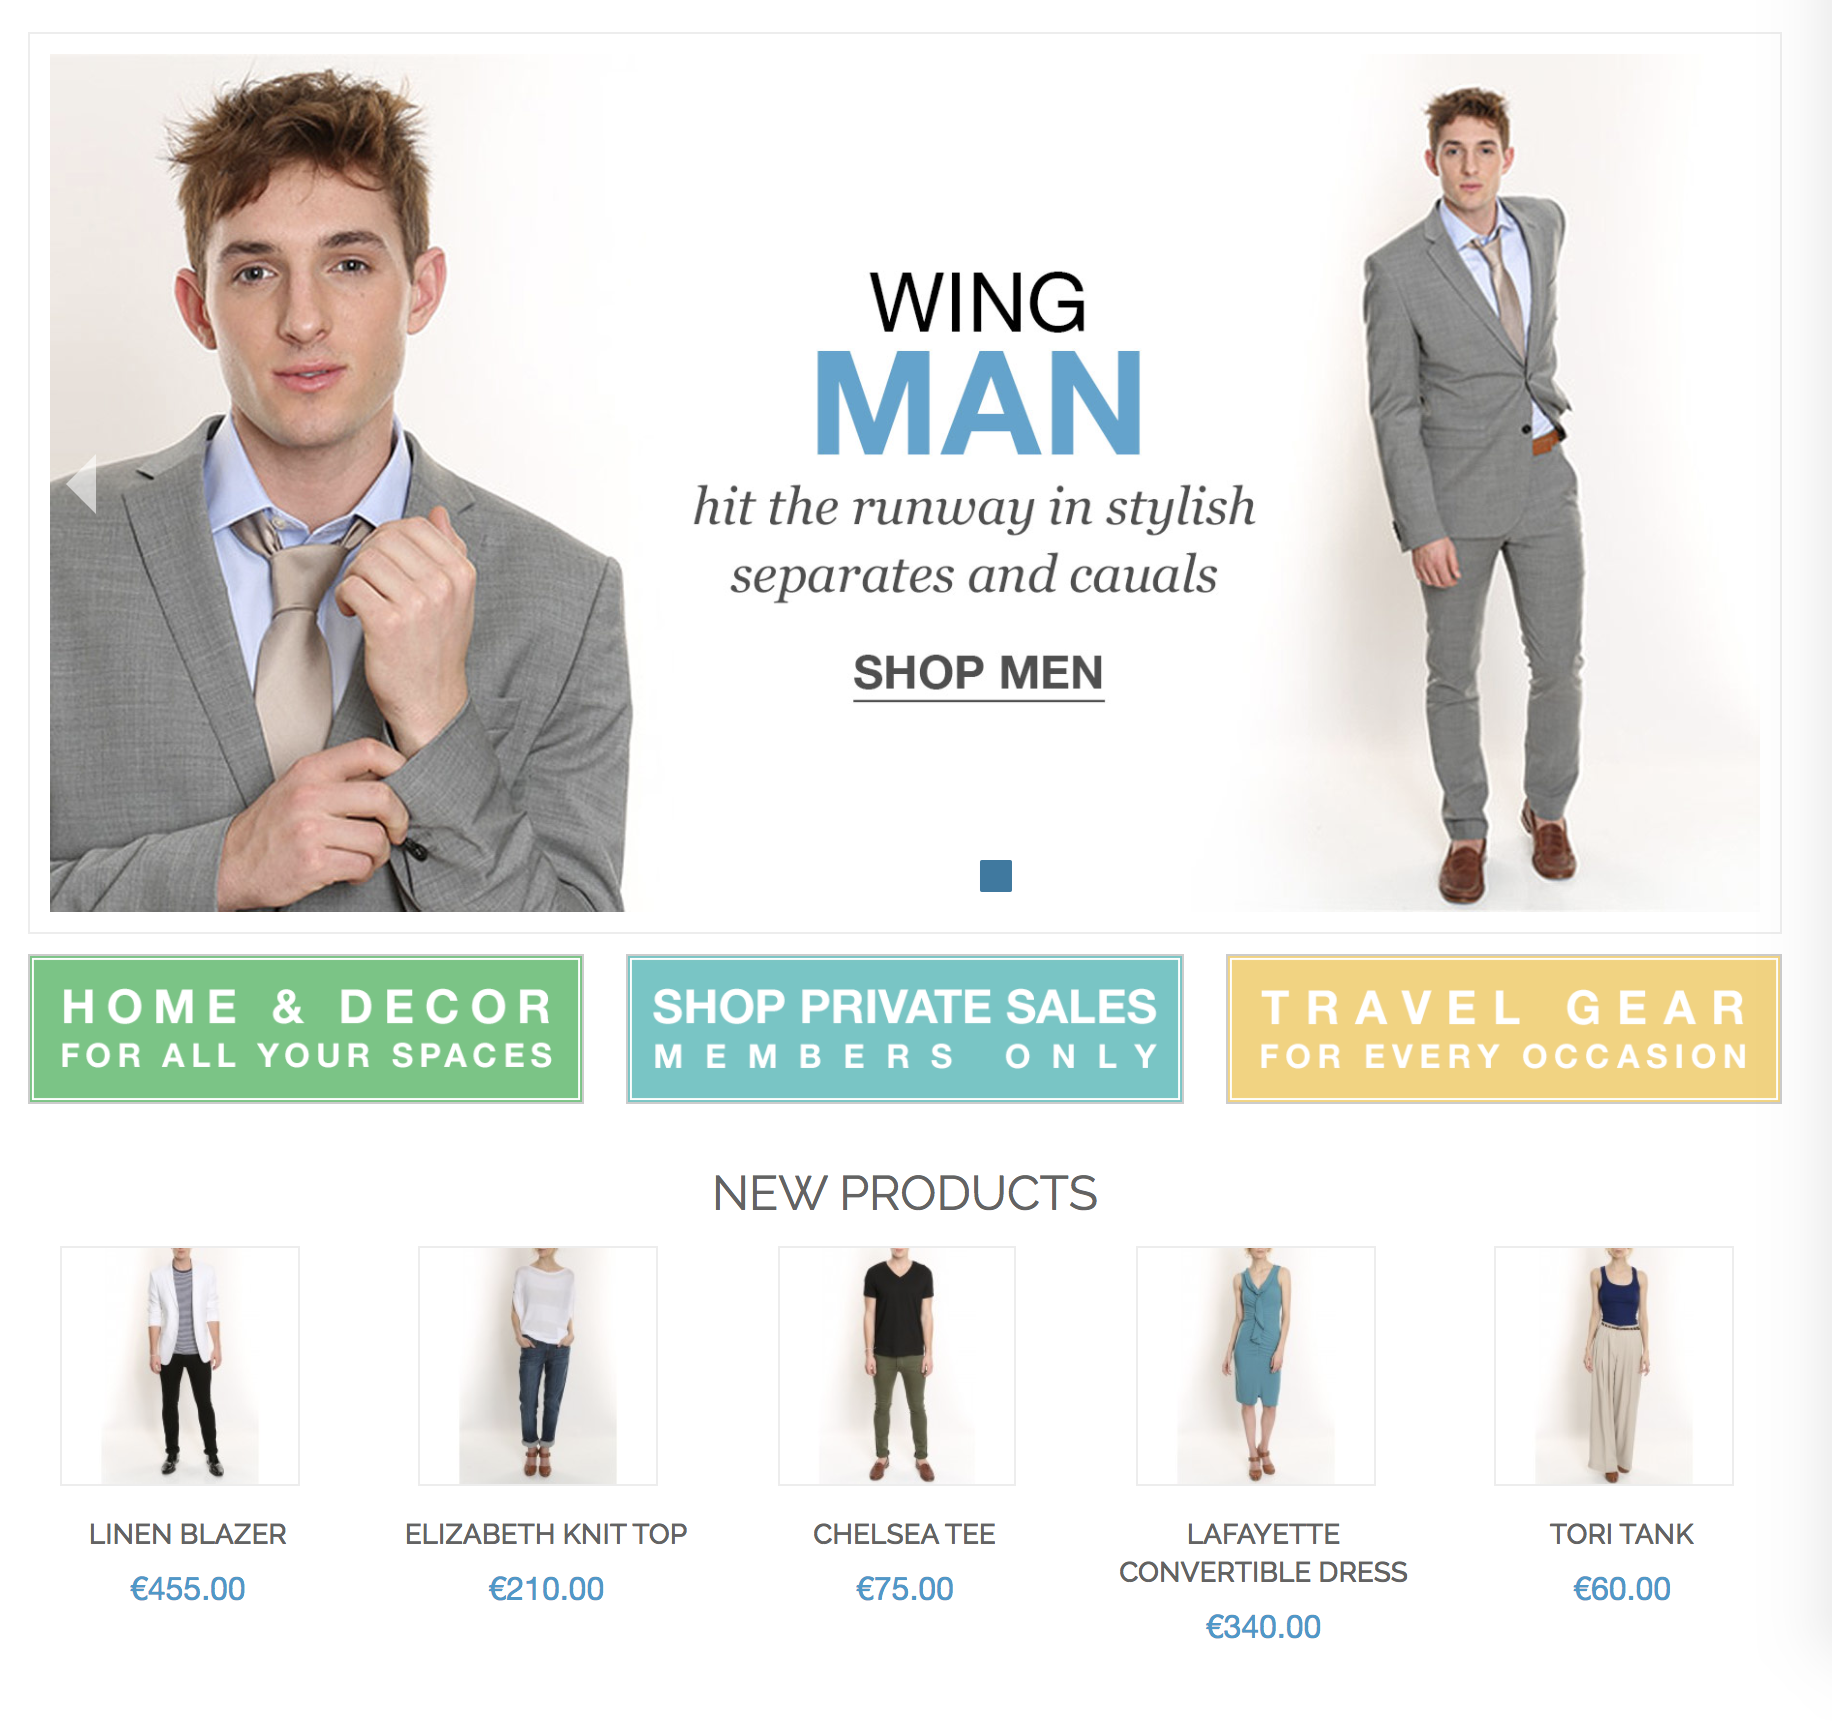
\includegraphics[height=7cm]{images/diagrams/before/desktop-homepage.png}
  \caption{Homepage Desktop Version}
  \label{fig:desktop-before-homepage}
\end{figure}
\vspace{0.5cm}

\begin{figure}[H]
  \centering
    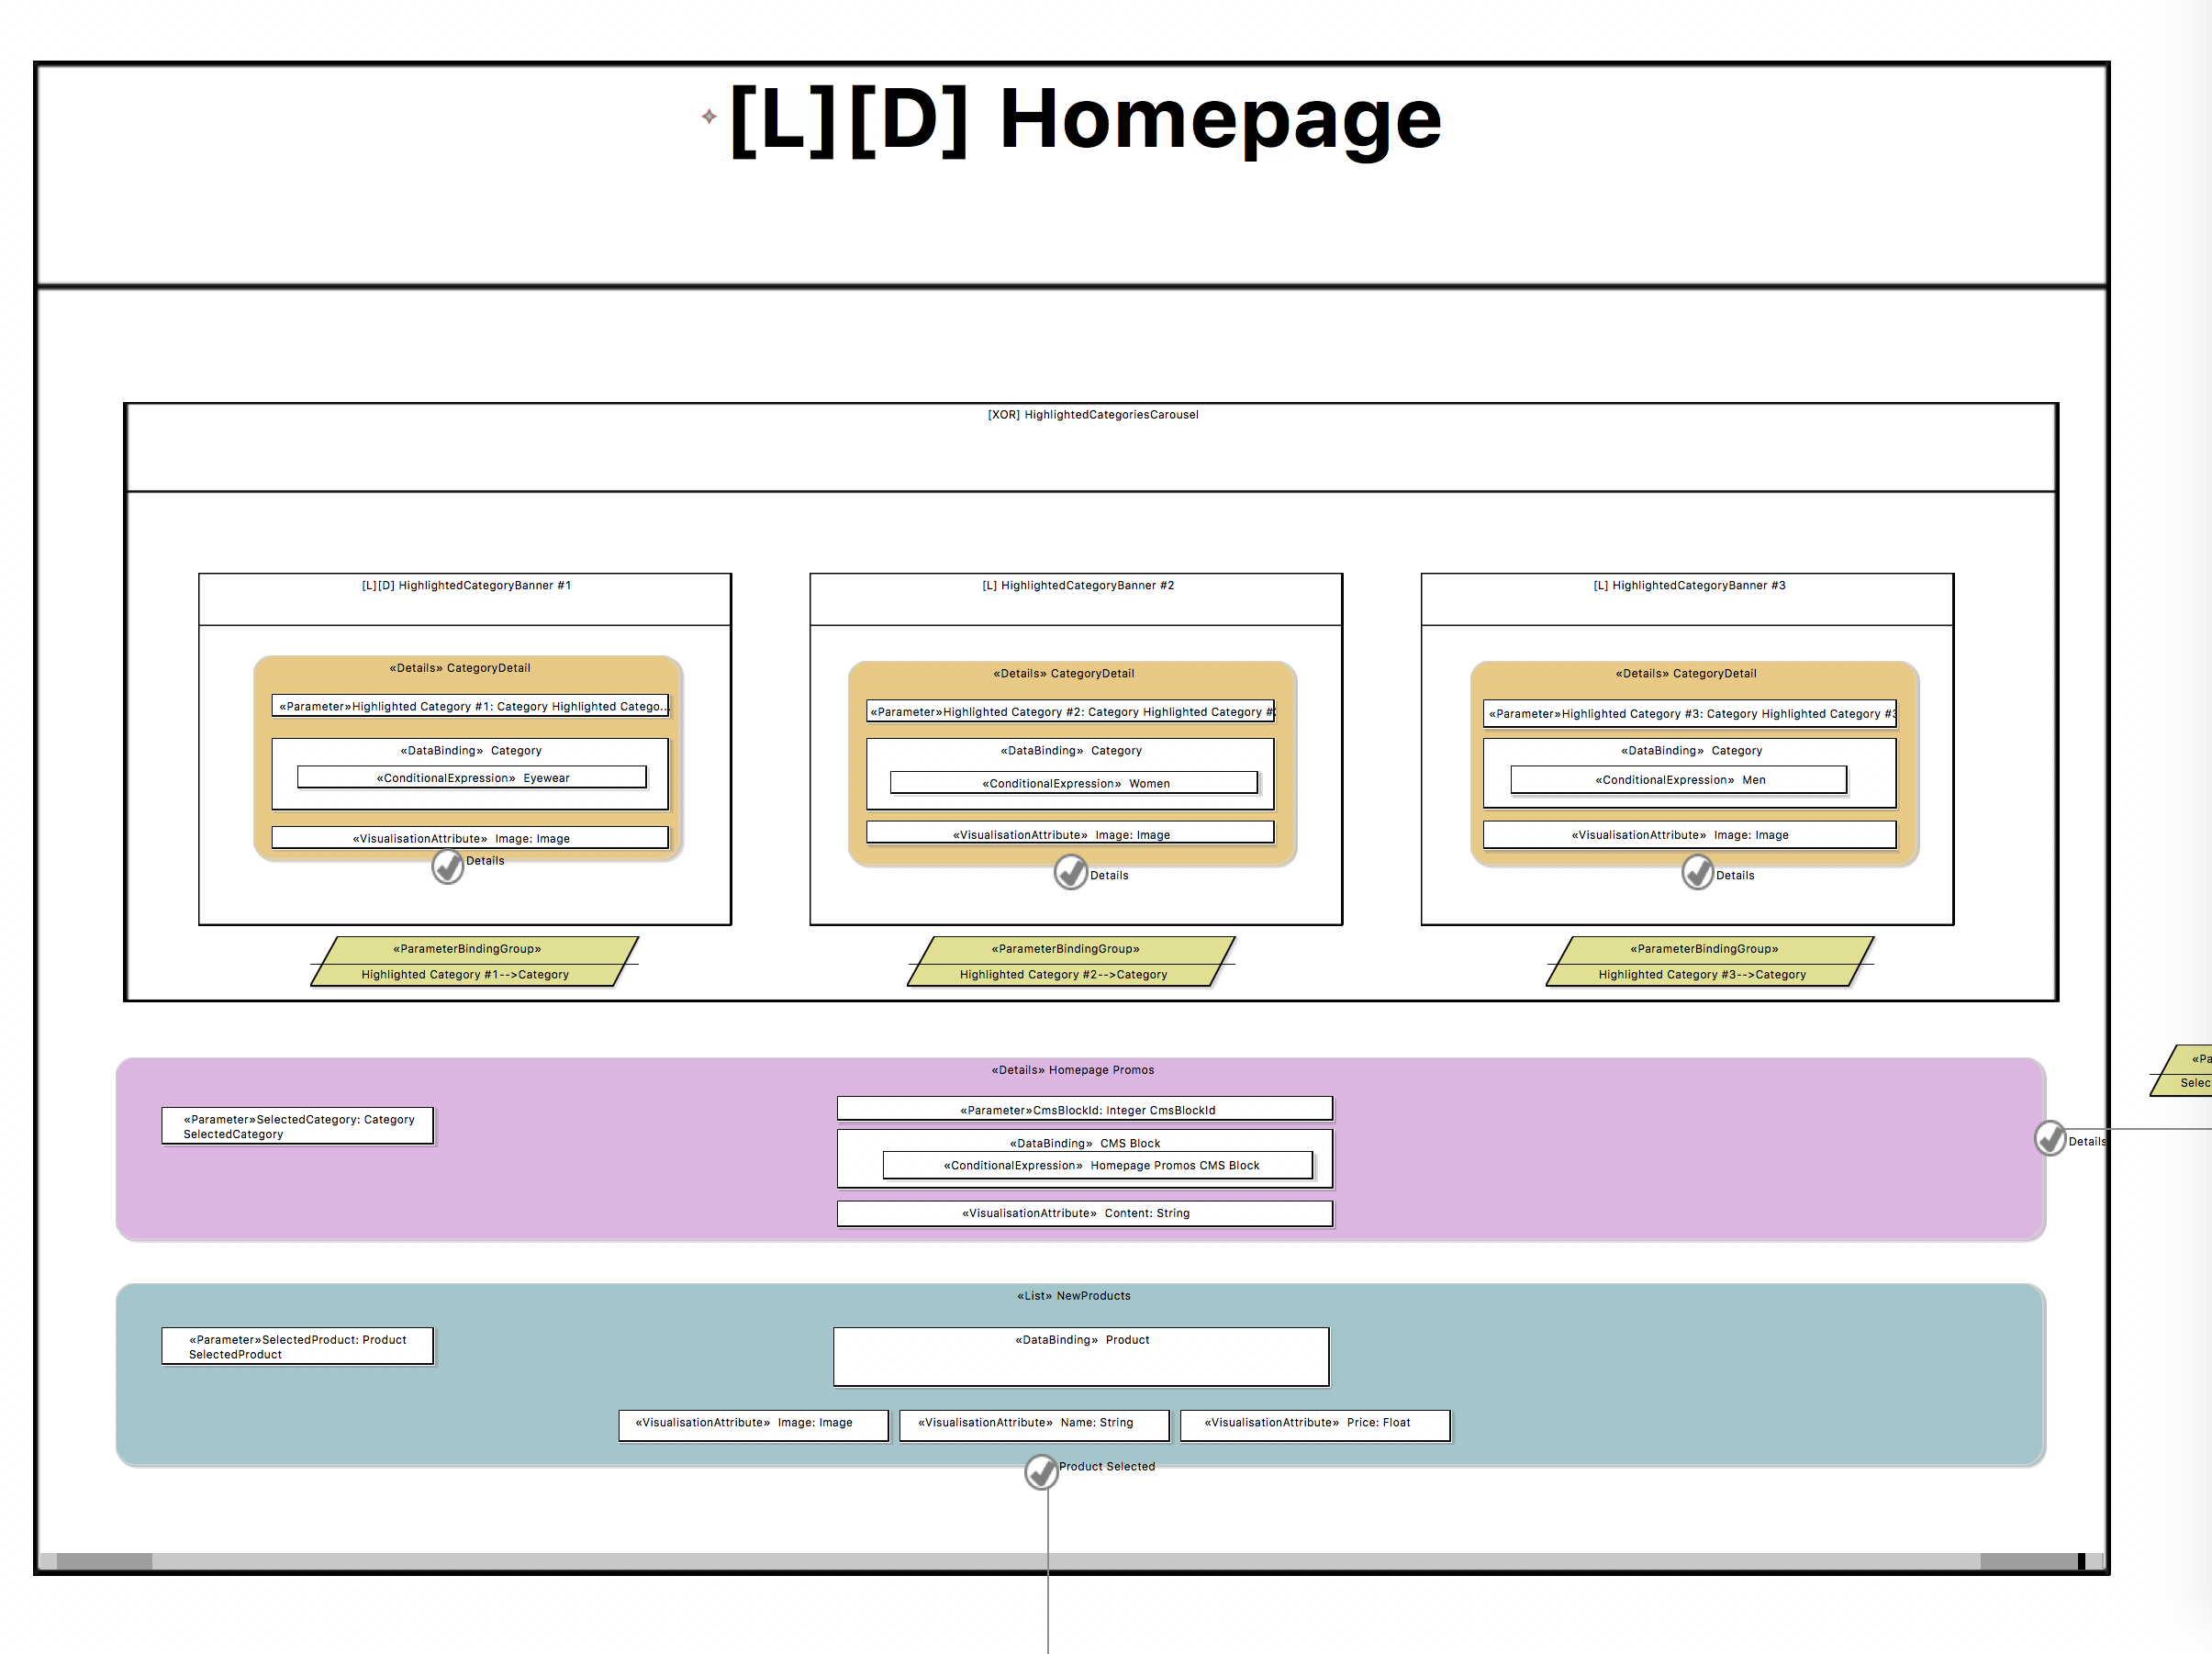
\includegraphics[height=7cm]{images/diagrams/before/ifml-homepage.png}
  \caption{Homepage IFML Diagram}
  \label{fig:ifml-before-homepage}
\end{figure}
\vspace{0.5cm}

\newpage
The following snippet of code is an extract from the IFML Model for the first \textit{HighlighedCategoryBanner View Container} element: 

\lstset{language=XML}
\begin{lstlisting} 
      <viewElements xsi:type="ext:Details"  name="CategoryDetail">
        <parameters  name="Highlighted Category #1" direction="inout">
          <constraints  language="SQL" body="Category.ID=18"/>
        </parameters>
        <viewElementEvents xsi:type="ext:OnSelectEvent"  name="Details" viewElement="//@interactionFlowModel/@interactionFlowModelElements.0/@viewElements.0/@viewElements.0">
          <outInteractionFlows xsi:type="core:NavigationFlow"  targetInteractionFlowElement="//@interactionFlowModel/@interactionFlowModelElements.6">
            <parameterBindingGroup >
              <parameterBindings  sourceParameter="//@interactionFlowModel/@interactionFlowModelElements.0/@viewElements.0/@viewElements.0/@viewElements.0/@parameters.0" targetParameter="//@interactionFlowModel/@interactionFlowModelElements.6/@parameters.0"/>
            </parameterBindingGroup>
          </outInteractionFlows>
        </viewElementEvents>
        <viewComponentParts xsi:type="core:DataBinding"  name="Category" uniformResourceIdentifier="">
          <subViewComponentParts xsi:type="core:ConditionalExpression"  language="SQL" body="Category.ID=18" name="Eyewear"/>
        </viewComponentParts>
        <viewComponentParts xsi:type="core:VisualizationAttribute"  name="Image" featureConcept="//@domainModel/@domainElements.4"/>
      </viewElements>
    </viewElements>
\end{lstlisting}

\newpage
The above snippet belongs to a more complex IFML model hierarchy as shown in \ref{fig:ifml-before-hierarchy-homepage}.

\vspace{0.5cm}
\begin{figure}[H]
  \centering
    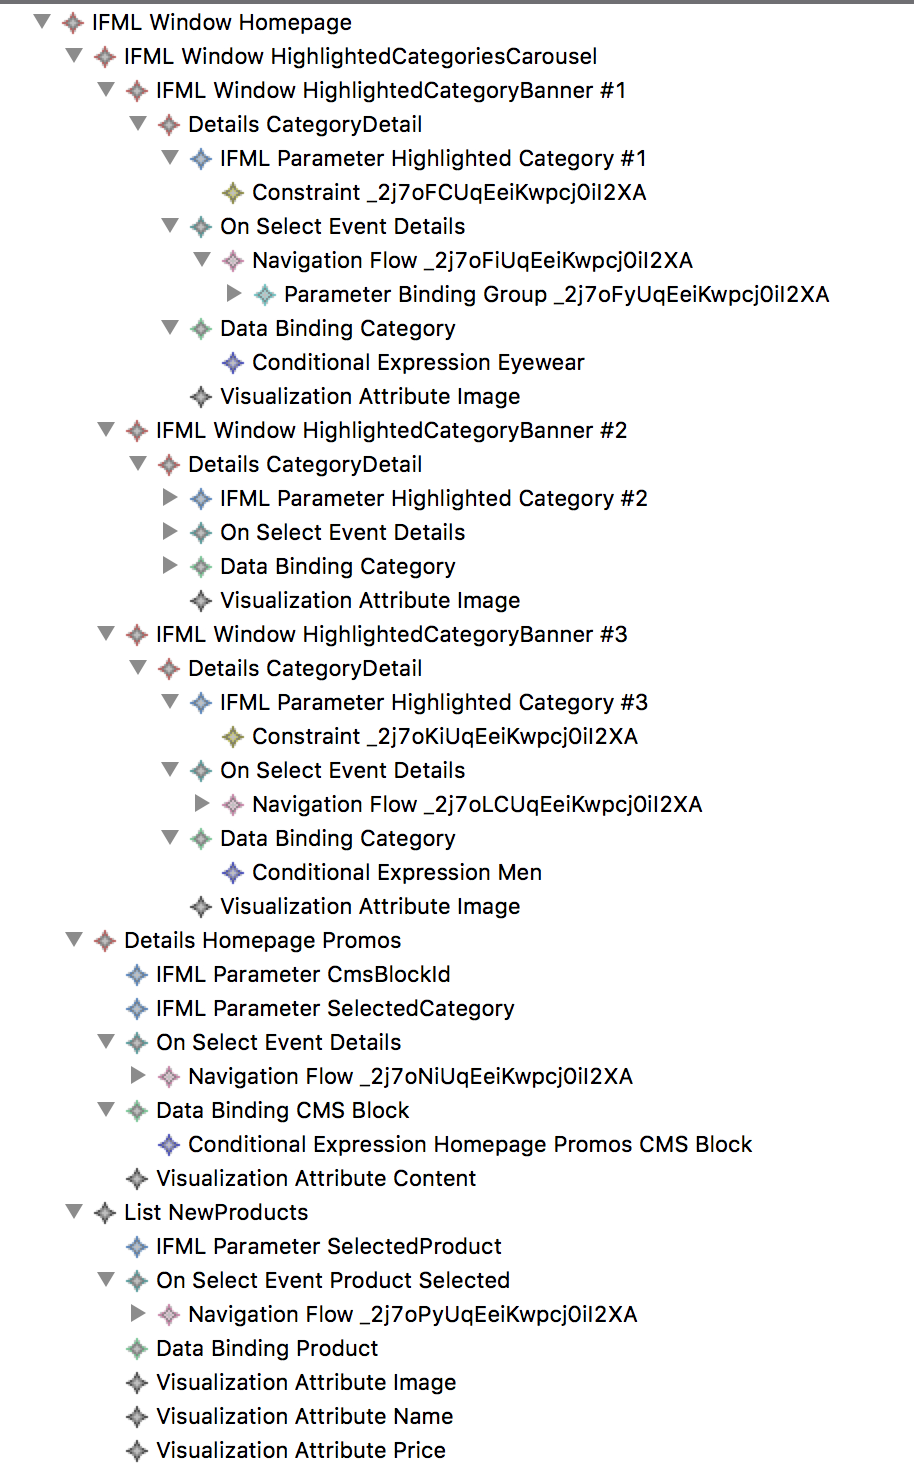
\includegraphics[height=12cm]{images/diagrams/before/ifml-hierarchy-homepage.png}
  \caption{Interaction Flow Homepage Model eCore representation}
  \label{fig:ifml-before-hierarchy-homepage}
\end{figure}
\vspace{0.5cm}

\subsubsection{Category Page overview}

The Madison Island Interaction Model for the Category Page (Figure \ref{fig:desktop-before-category} and \ref{fig:ifml-before-category}) is composed by a parent \textit{IFMLWindow} element in \textit{XOR mode} which presents information about the current category on the top of the page. Depending on the display mode property for the Category Entity, the user can be presented with two different \textit{View Containers} that are respectively activated using different \textit{Activation Expressions} based on the value of the property itself. Whilst the first scenario presents a \textit{Detail View Component} attached to a linked CMS Block, the second option shows two children view components representing both the filter sidebar and the products listing section with this last one having multiple \textit{Visualization Attribute} children nodes indicating the user is presented with an image used as thumbnail, a name and a price for each product belonging to the category shown.

\vspace{0.5cm}
\begin{figure}[H]
  \centering
  \subfloat[Display Mode PAGE]{{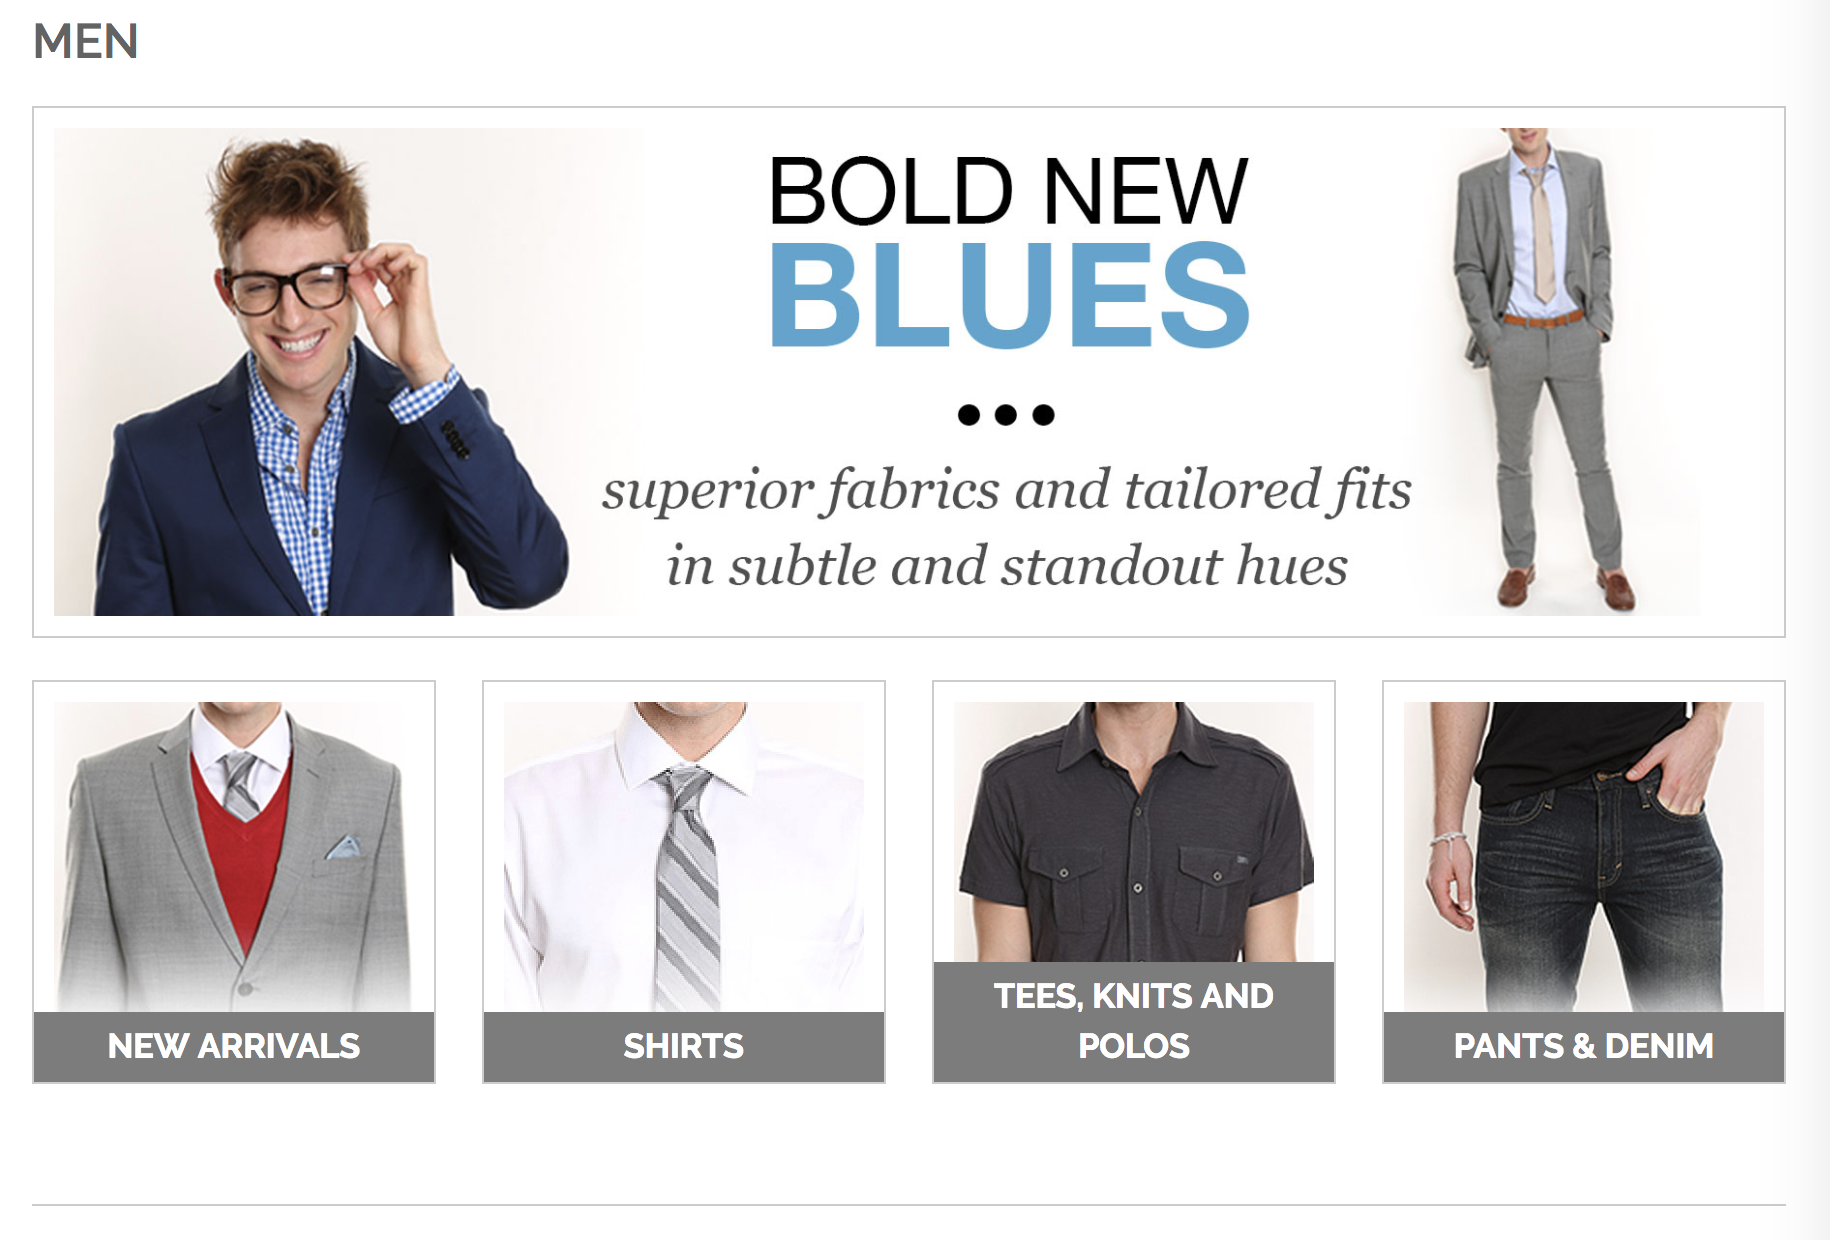
\includegraphics[width=7cm]{images/diagrams/before/desktop-category1.png} }}%
  \qquad
  \subfloat[Display Mode PRODUCTS]{{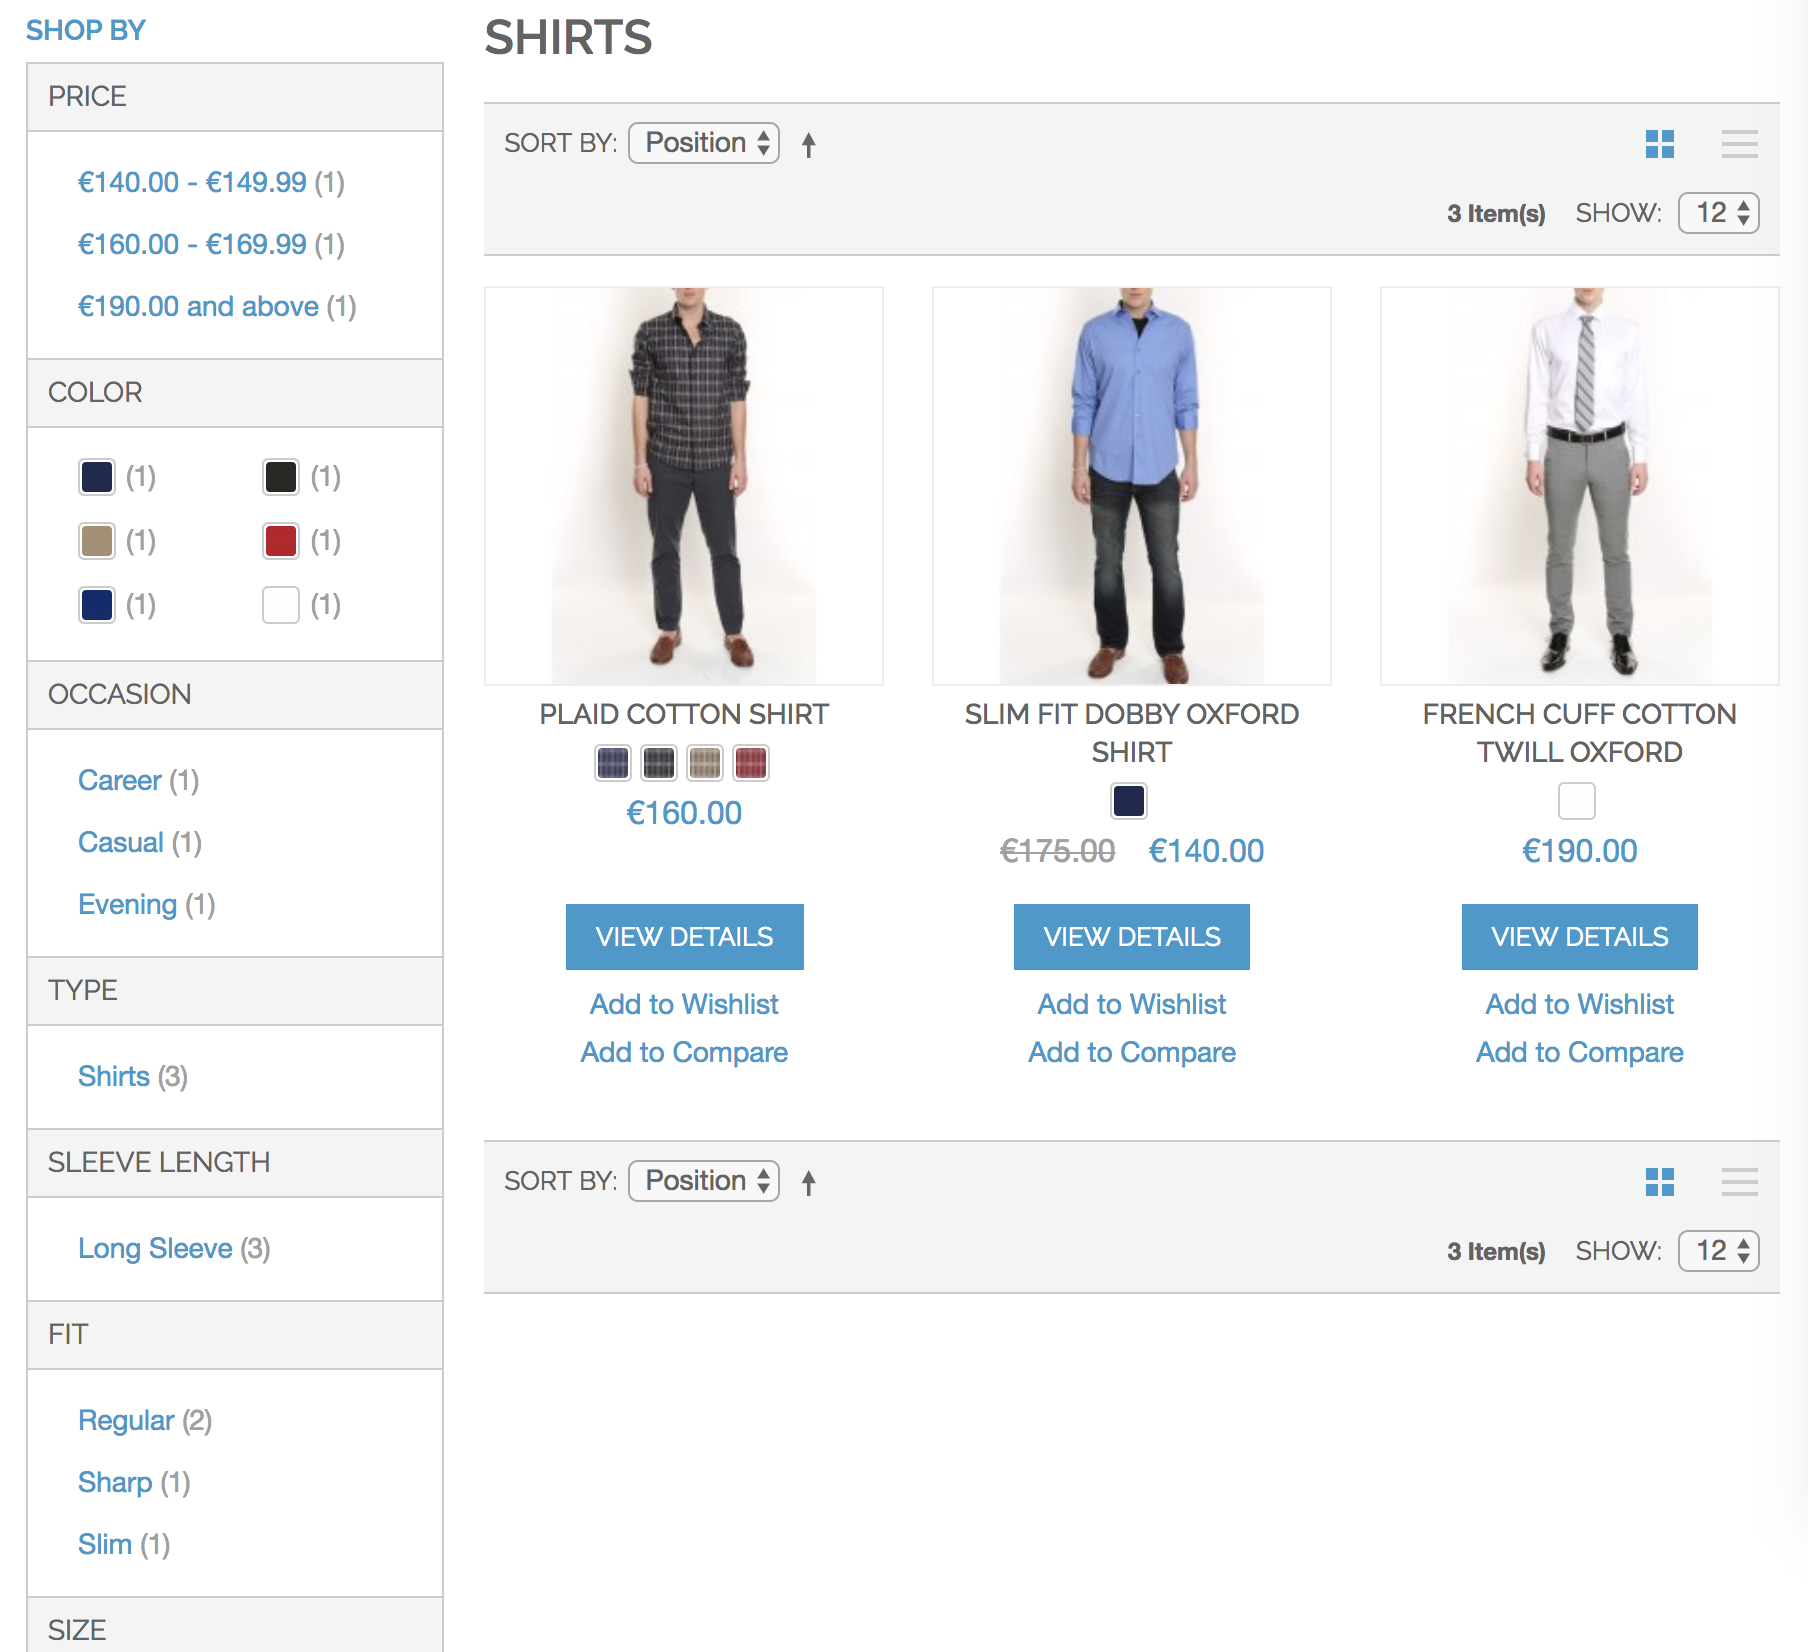
\includegraphics[width=7cm]{images/diagrams/before/desktop-category2.png} }}%
  \caption{Category Desktop Versions}%
  \label{fig:desktop-before-category}%
\end{figure}

\begin{figure}[H]
  \centering
    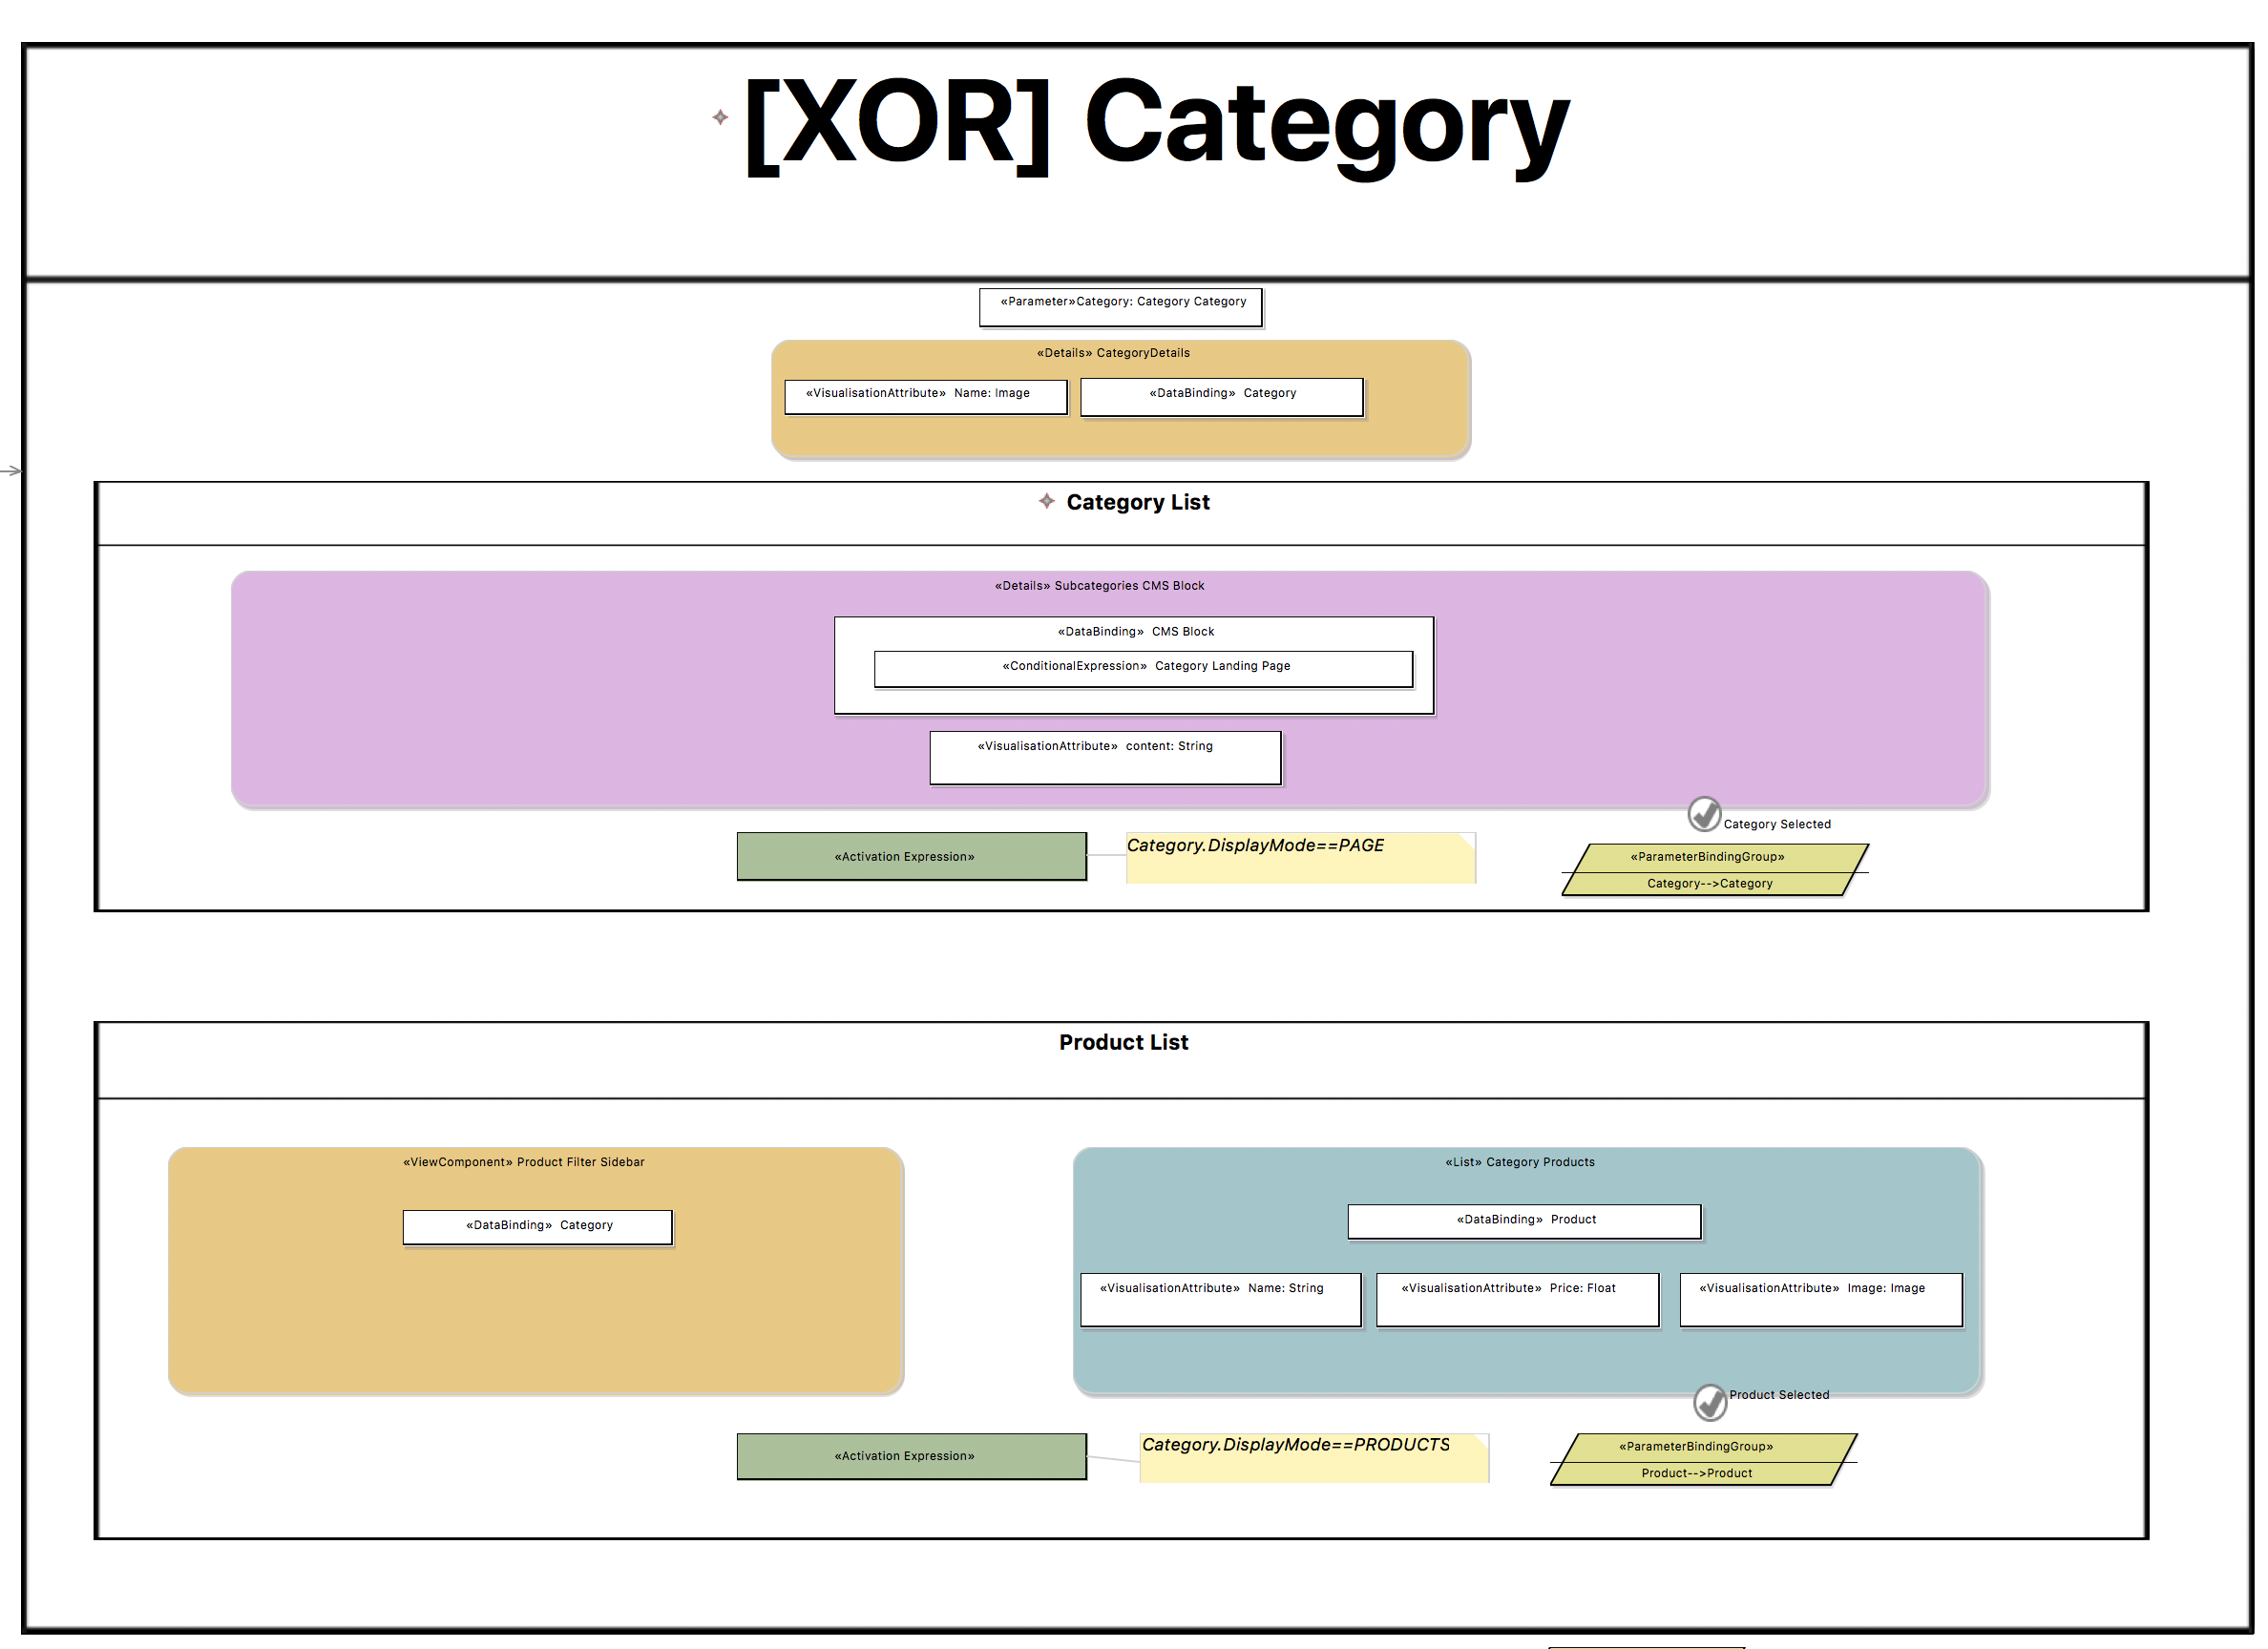
\includegraphics[height=10cm]{images/diagrams/before/ifml-category.png}
  \caption{Category IFML Diagram}
  \label{fig:ifml-before-category}
\end{figure}
\vspace{0.5cm}

The IFML Model code for the first \textit{Category Products List} element we just described has this form: 

\lstset{language=XML}
\begin{lstlisting} 
    <viewElements xsi:type="ext:List"  name="Category Products">
    <viewElementEvents xsi:type="ext:OnSelectEvent"  name="Product Selected" viewElement="//@interactionFlowModel/@interactionFlowModelElements.6/@viewElements.1/@viewElements.0">
      <outInteractionFlows xsi:type="core:NavigationFlow"  targetInteractionFlowElement="//@interactionFlowModel/@interactionFlowModelElements.1">
        <parameterBindingGroup >
          <parameterBindings  sourceParameter="//@interactionFlowModel/@interactionFlowModelElements.1/@parameters.0" targetParameter="//@interactionFlowModel/@interactionFlowModelElements.1/@parameters.0"/>
        </parameterBindingGroup>
      </outInteractionFlows>
    </viewElementEvents>
    <viewComponentParts xsi:type="core:DataBinding"  name="Product" domainConcept="//@domainModel/@domainElements.3">
      <conditionalExpression  language="SQL" body="Category IN Product.Categories" name="Category Products"/>
    </viewComponentParts>
    <viewComponentParts xsi:type="core:VisualizationAttribute"  name="Image" featureConcept="//@domainModel/@domainElements.7"/>
    <viewComponentParts xsi:type="core:VisualizationAttribute"  name="Name" featureConcept="//@domainModel/@domainElements.8"/>
    <viewComponentParts xsi:type="core:VisualizationAttribute"  name="Price" featureConcept="//@domainModel/@domainElements.9"/>
  </viewElements>
  <viewElements xsi:type="core:ViewComponent"  name="Product Filter Sidebar">
    <viewComponentParts xsi:type="core:DataBinding"  name="Category"/>
  </viewElements>
</viewElements>
\end{lstlisting}

\newpage
The full expanded model hierarchy for the \textit{IFMLWindow} Category element is shown in Figure \ref{fig:ifml-before-hierarchy-category}.

\vspace{0.5cm}
\begin{figure}[H]
  \centering
    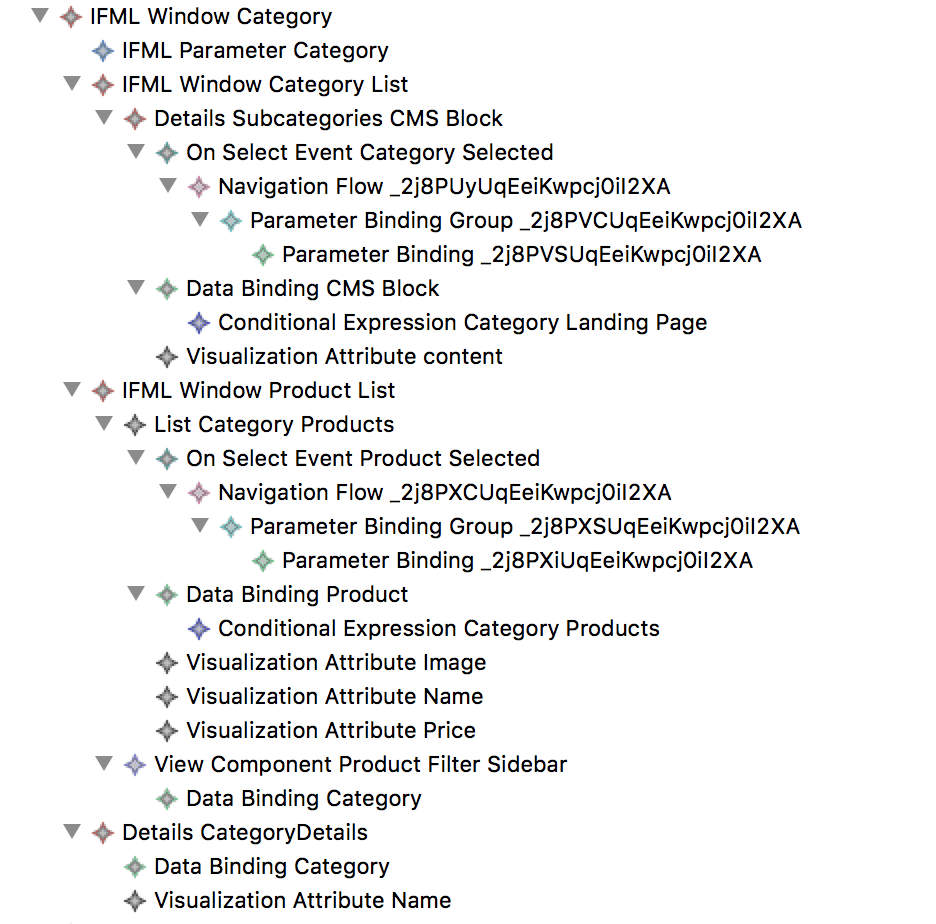
\includegraphics[width=13cm]{images/diagrams/before/ifml-hierarchy-category.png}
  \caption{Interaction Flow Category Model eCore representation}
  \label{fig:ifml-before-hierarchy-category}
\end{figure}
\vspace{0.5cm}


\subsubsection{Product Page overview}

The Madison Island Interaction Model for the Product page (Figure \ref{fig:desktop-before-product} and \ref{fig:ifml-before-product}) is mainly built with a single \textit{IFMLWindow} element containing different types of \textit{View Component} nodes with the main one being a Detail type one bound to the current product data entity. The other two elements are the single \textit{Form View Component} descibing the Add to Cart section and its possible interactions and the \textit{List View Component} holding the information for the Related Product widget.

\newpage
\vspace{0.5cm}
\begin{figure}[H]
  \centering
    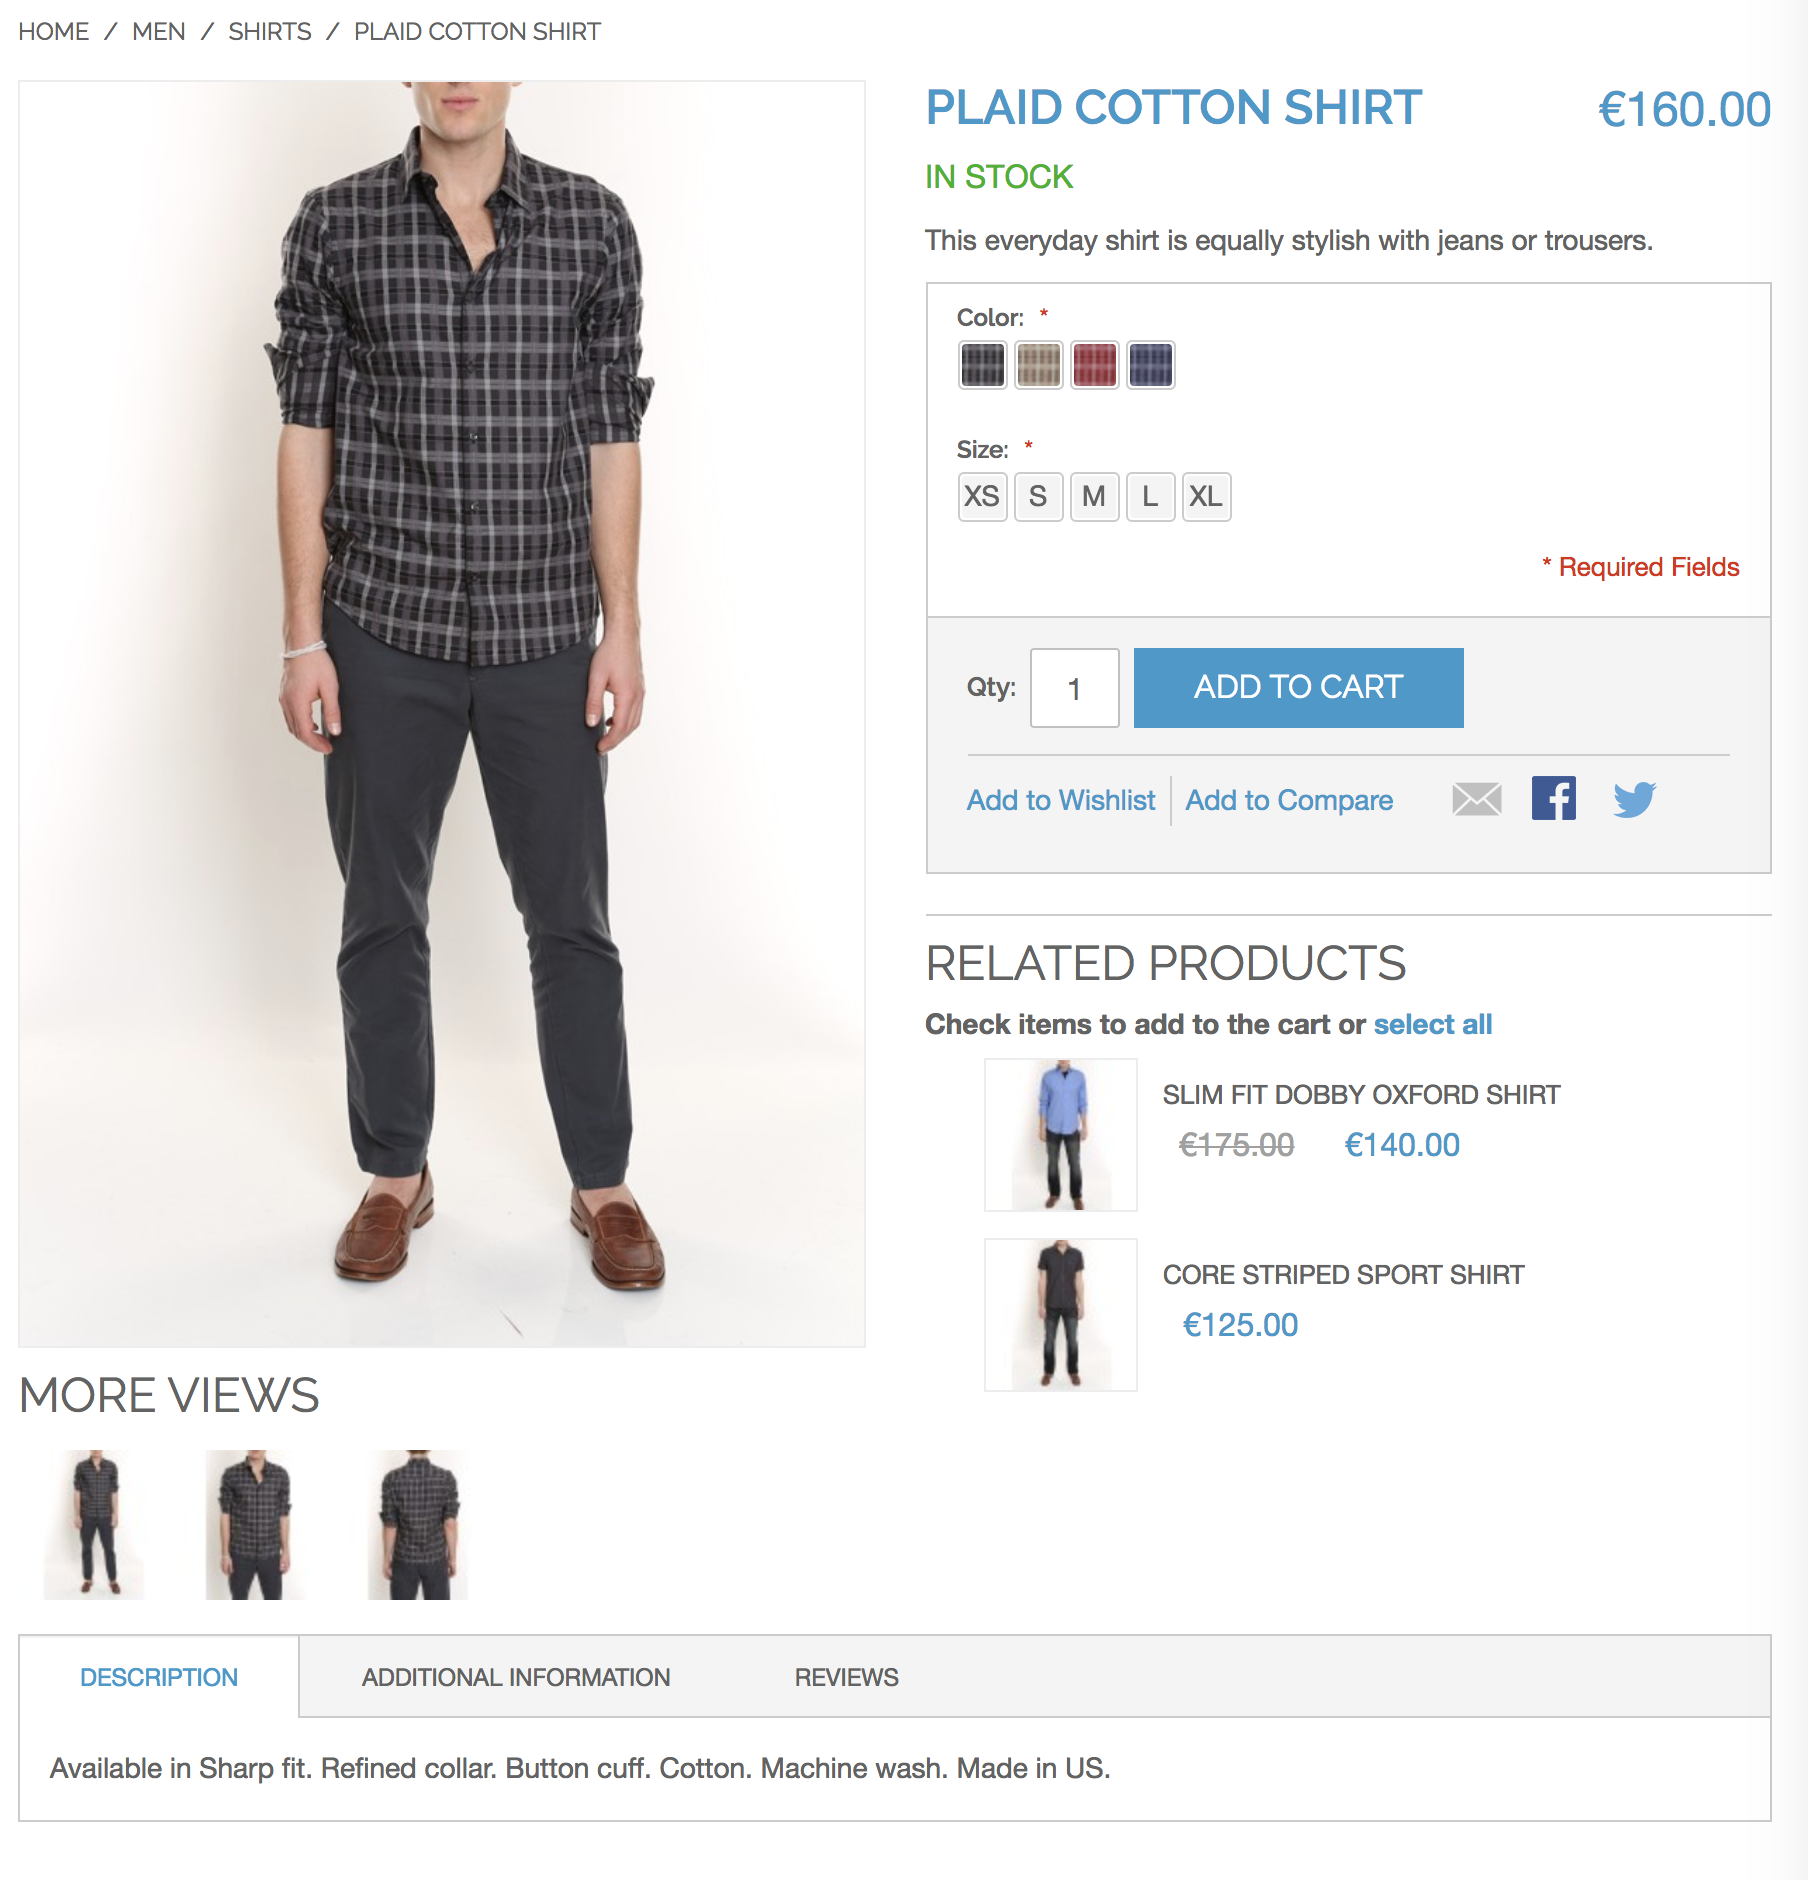
\includegraphics[height=10cm]{images/diagrams/before/desktop-product.png}
  \caption{Product Page Desktop Version}
  \label{fig:desktop-before-product}
\end{figure}

\vspace{0.5cm}
\begin{figure}[H]
  \centering
    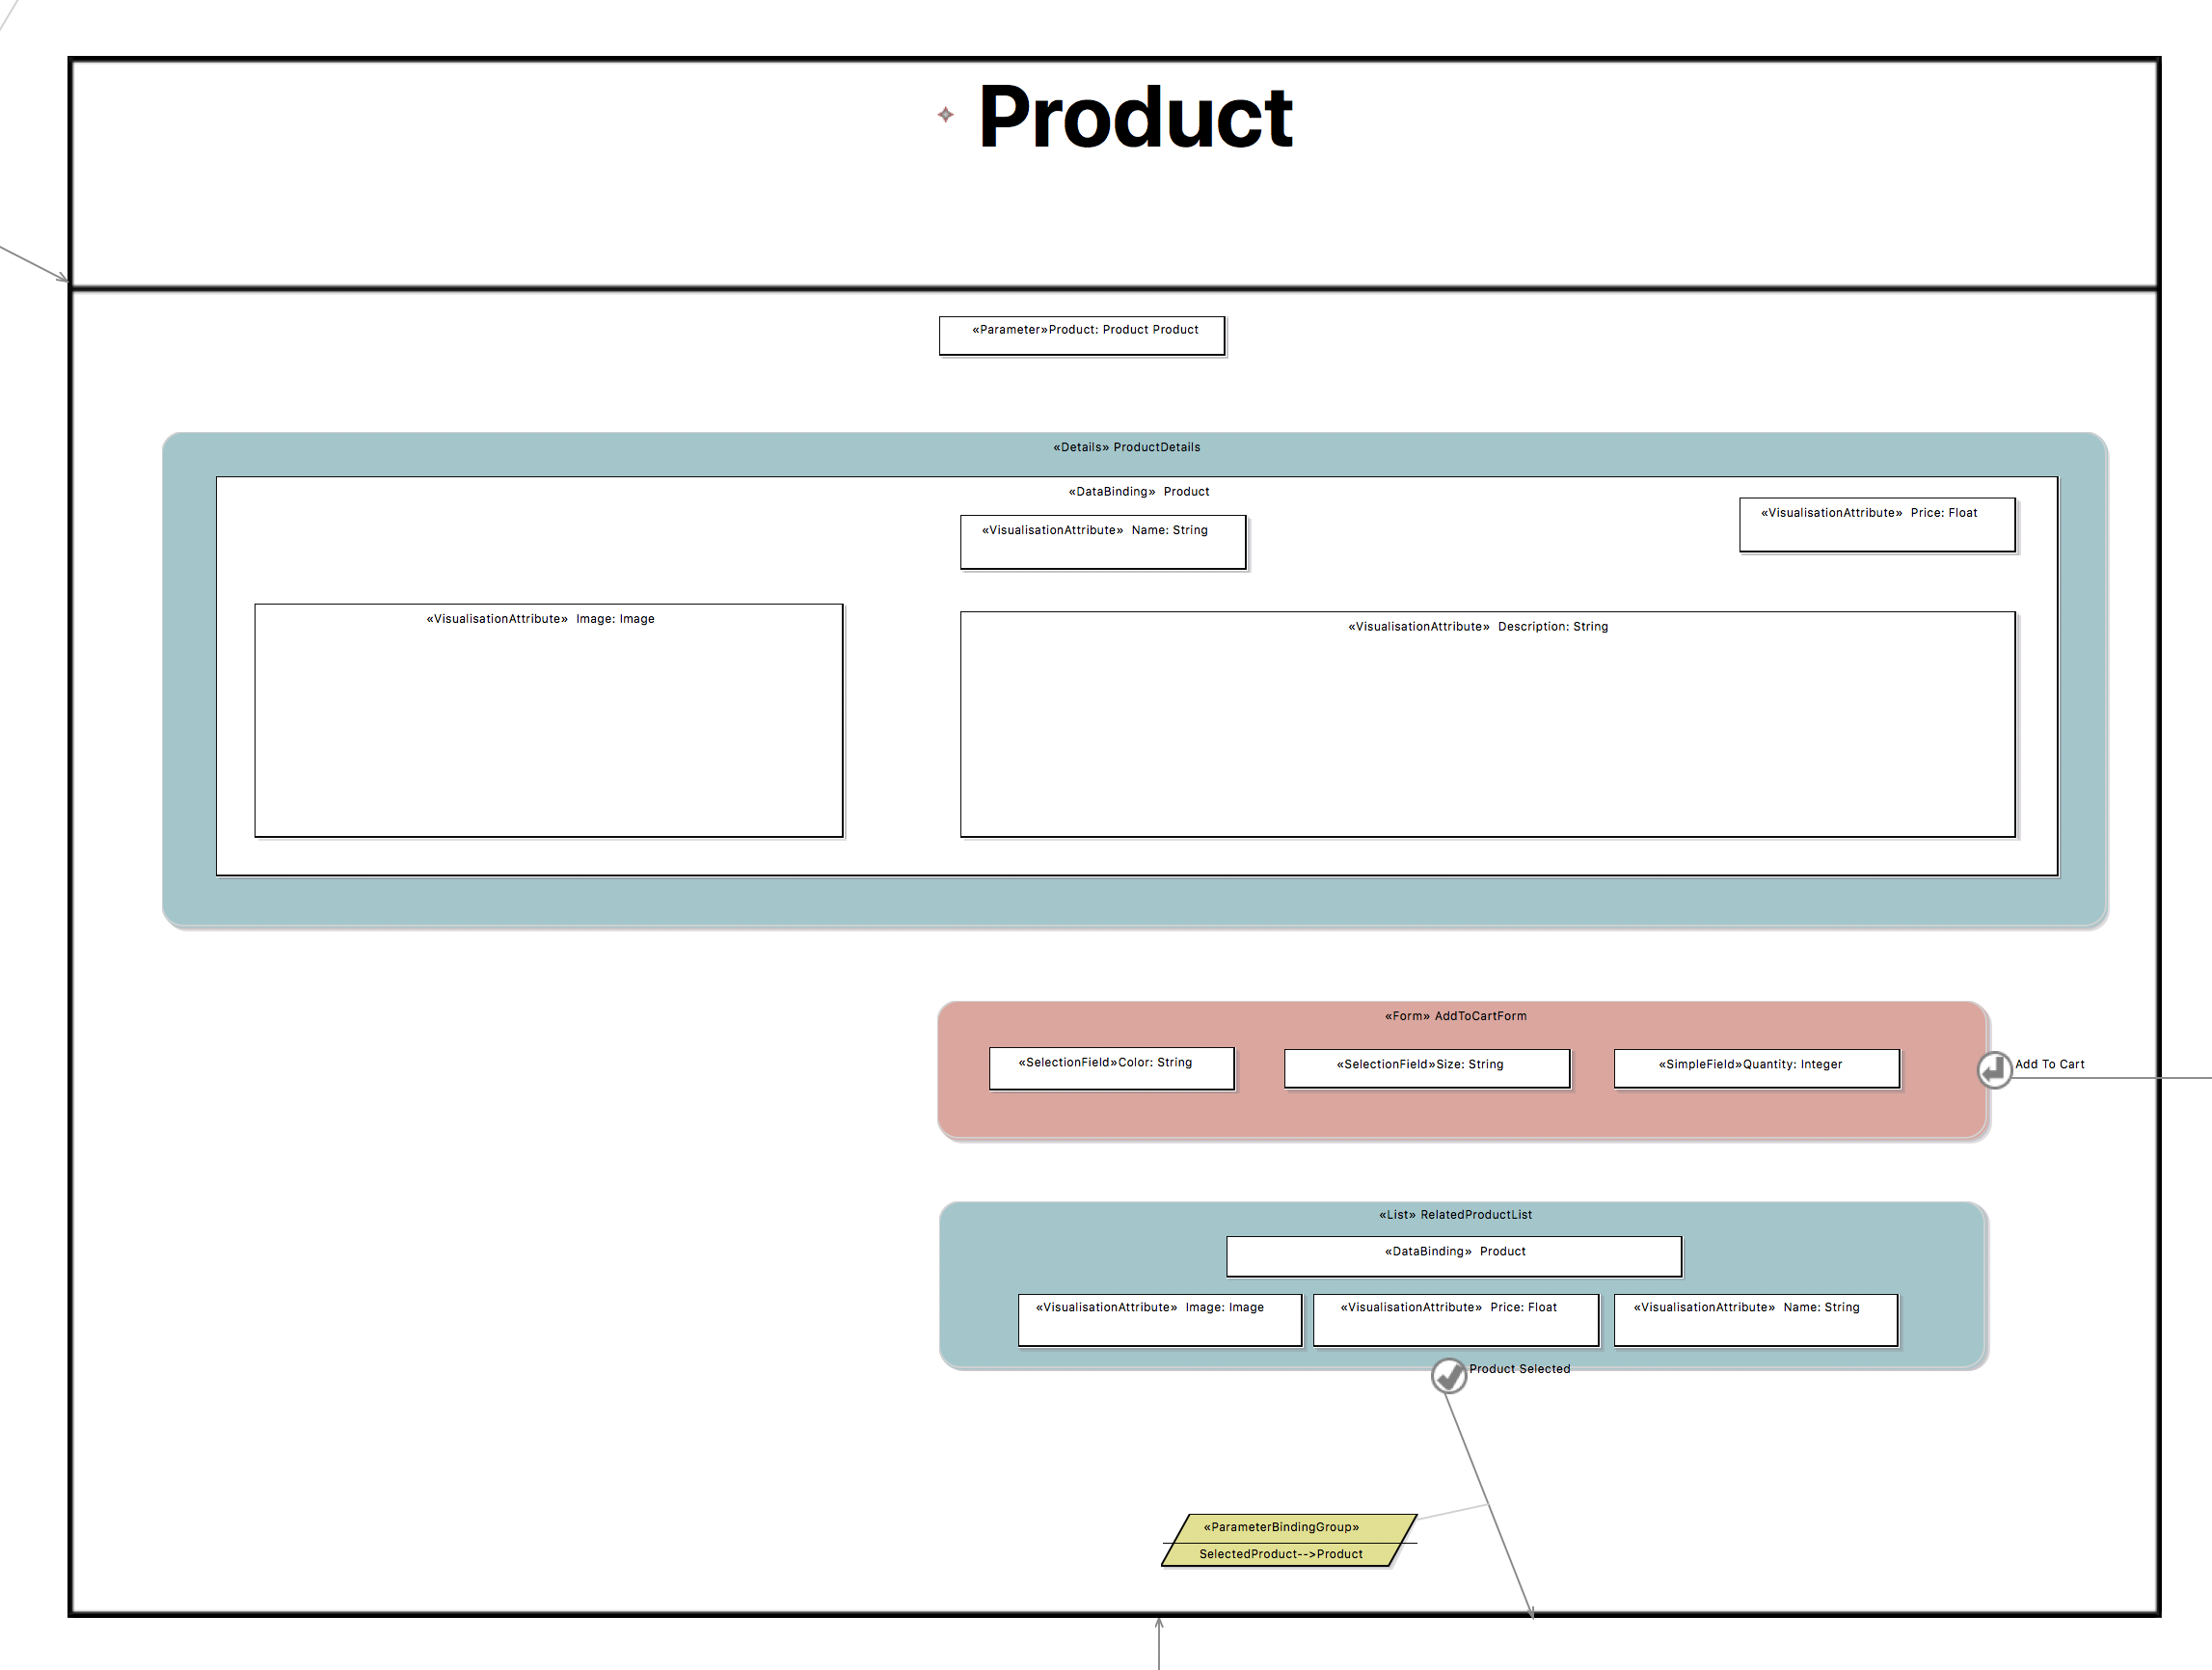
\includegraphics[height=10cm]{images/diagrams/before/ifml-product.png}
  \caption{Product Page IFML Diagram}
  \label{fig:ifml-before-product}
\end{figure}
\vspace{0.5cm}

\newpage
The structure of the model just outlined produces the following IFMLModel code:

\lstset{language=XML}
\begin{lstlisting} 
    <interactionFlowModelElements xsi:type="ext:IFMLWindow"  name="Product" inInteractionFlows="//@interactionFlowModel/@interactionFlowModelElements.1/@viewElements.2/@viewElementEvents.0/@outInteractionFlows.0 //@interactionFlowModel/@interactionFlowModelElements.0/@viewElements.2/@viewElementEvents.0/@outInteractionFlows.0 //@interactionFlowModel/@interactionFlowModelElements.10/@viewElements.0/@viewElementEvents.0/@outInteractionFlows.0 //@interactionFlowModel/@interactionFlowModelElements.6/@viewElements.1/@viewElements.0/@viewElementEvents.0/@outInteractionFlows.0">
      <parameters  name="Product" />
      <viewElements xsi:type="ext:Details"  name="ProductDetails">
        <viewComponentParts xsi:type="core:DataBinding"  name="Product" uniformResourceIdentifier="">
          <subViewComponentParts xsi:type="core:VisualizationAttribute"  name="Price" featureConcept="//@domainModel/@domainElements.9"/>
          <subViewComponentParts xsi:type="core:VisualizationAttribute"  name="Image" featureConcept="//@domainModel/@domainElements.7"/>
          <subViewComponentParts xsi:type="core:VisualizationAttribute"  name="Name" featureConcept="//@domainModel/@domainElements.8"/>
          <subViewComponentParts xsi:type="core:VisualizationAttribute"  name="Description" featureConcept="//@domainModel/@domainElements.10"/>
        </viewComponentParts>
      </viewElements>
      <viewElements xsi:type="ext:Form"  name="AddToCartForm">
        <viewElementEvents xsi:type="ext:OnSubmitEvent"  name="Add To Cart" viewElement="//@interactionFlowModel/@interactionFlowModelElements.1/@viewElements.1">
          <outInteractionFlows xsi:type="core:NavigationFlow"  targetInteractionFlowElement="//@interactionFlowModel/@interactionFlowModelElements.9">
            <parameterBindingGroup >
              <parameterBindings  sourceParameter="//@interactionFlowModel/@interactionFlowModelElements.1/@viewElements.1/@viewComponentParts.2" targetParameter="//@interactionFlowModel/@interactionFlowModelElements.1/@viewElements.1/@viewComponentParts.2"/>
            </parameterBindingGroup>
          </outInteractionFlows>
        </viewElementEvents>
        <viewComponentParts xsi:type="ext:SelectionField"  name="Color" />
        <viewComponentParts xsi:type="ext:SelectionField"  name="Size" />
        <viewComponentParts xsi:type="ext:SimpleField"  name="Quantity" />
      </viewElements>
      <viewElements xsi:type="ext:List"  name="RelatedProductList">
        <viewElementEvents xsi:type="ext:OnSelectEvent"  name="Product Selected" viewElement="//@interactionFlowModel/@interactionFlowModelElements.1/@viewElements.2">
          <outInteractionFlows xsi:type="core:NavigationFlow"  targetInteractionFlowElement="//@interactionFlowModel/@interactionFlowModelElements.1">
            <parameterBindingGroup >
              <parameterBindings  sourceParameter="//@interactionFlowModel/@interactionFlowModelElements.0/@viewElements.2/@parameters.0" targetParameter="//@interactionFlowModel/@interactionFlowModelElements.1/@parameters.0"/>
            </parameterBindingGroup>
          </outInteractionFlows>
        </viewElementEvents>
        <viewComponentParts xsi:type="core:DataBinding"  name="Product"/>
        <viewComponentParts xsi:type="core:VisualizationAttribute"  name="Image" featureConcept="//@domainModel/@domainElements.7"/>
        <viewComponentParts xsi:type="core:VisualizationAttribute"  name="Name" featureConcept="//@domainModel/@domainElements.8"/>
        <viewComponentParts xsi:type="core:VisualizationAttribute"  name="Price" featureConcept="//@domainModel/@domainElements.9"/>
      </viewElements>
    </interactionFlowModelElements>
\end{lstlisting}

\newpage
The model representation of this Product page structure is shown in Figure \ref{fig:ifml-before-hierarchy-product}

\vspace{0.5cm}
\begin{figure}[H]
  \centering
    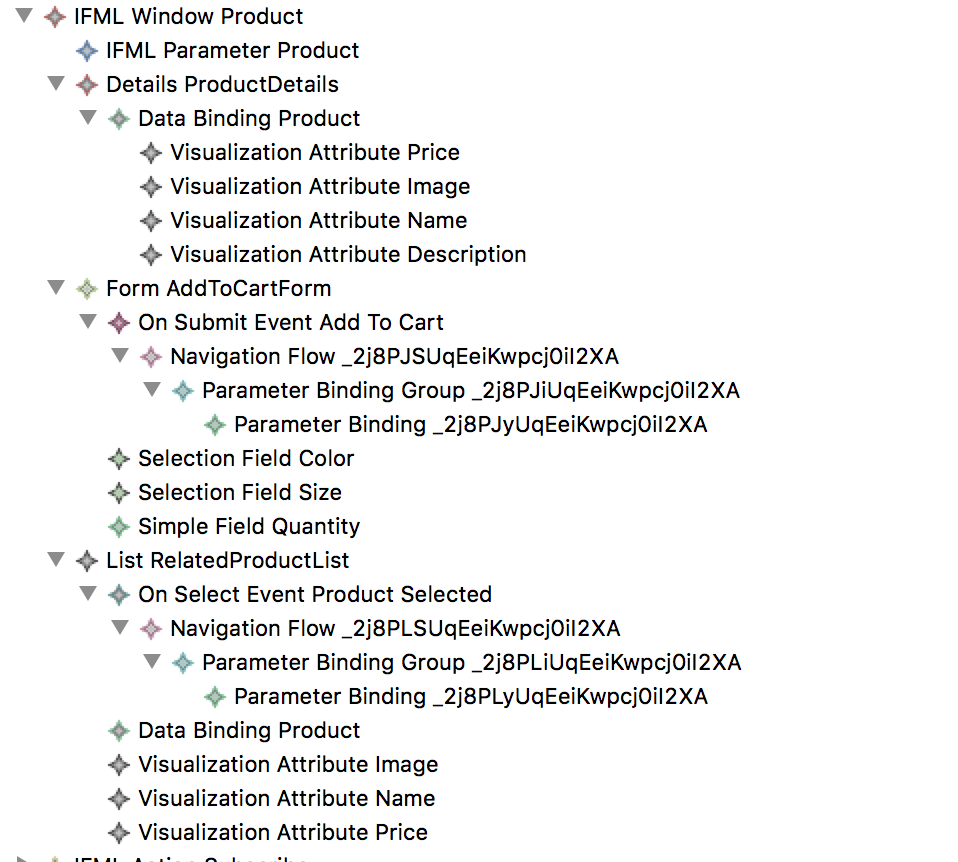
\includegraphics[width=13cm]{images/diagrams/before/ifml-hierarchy-product.png}
  \caption{Interaction Flow Product Model eCore representation}
  \label{fig:ifml-before-hierarchy-product}
\end{figure}
\vspace{0.5cm}

\subsubsection{Shopping Cart Page overview}

The Madison Island Interaction Model for the Shopping Cart page (Figure \ref{fig:desktop-before-shoppingcart} and \ref{fig:ifml-before-shoppingcart}) is  built with a single \textit{IFMLWindow} landmark container (flagging it as accessible from everywhere) including multiple \textit{Form View Component} instances representing the sidebar interactions with the discount codes and shipping estimation widgets. Besides the sidebar, the area with the cart status and the items in the cart is shown with another \textit{Form View Component} controlled by the \textit{Activation Condition} responsible for showing items when cart is not empty only. The area is modeled with a Form component because of the Qty input text fields which allow the user to update the related item quantities or empty the whole cart at any time. Both these interactions are controlled with specific \textit{IFMLAction} elements triggered on these \textit{Events}.

\newpage
\vspace{0.5cm}
\begin{figure}[H]
  \centering
    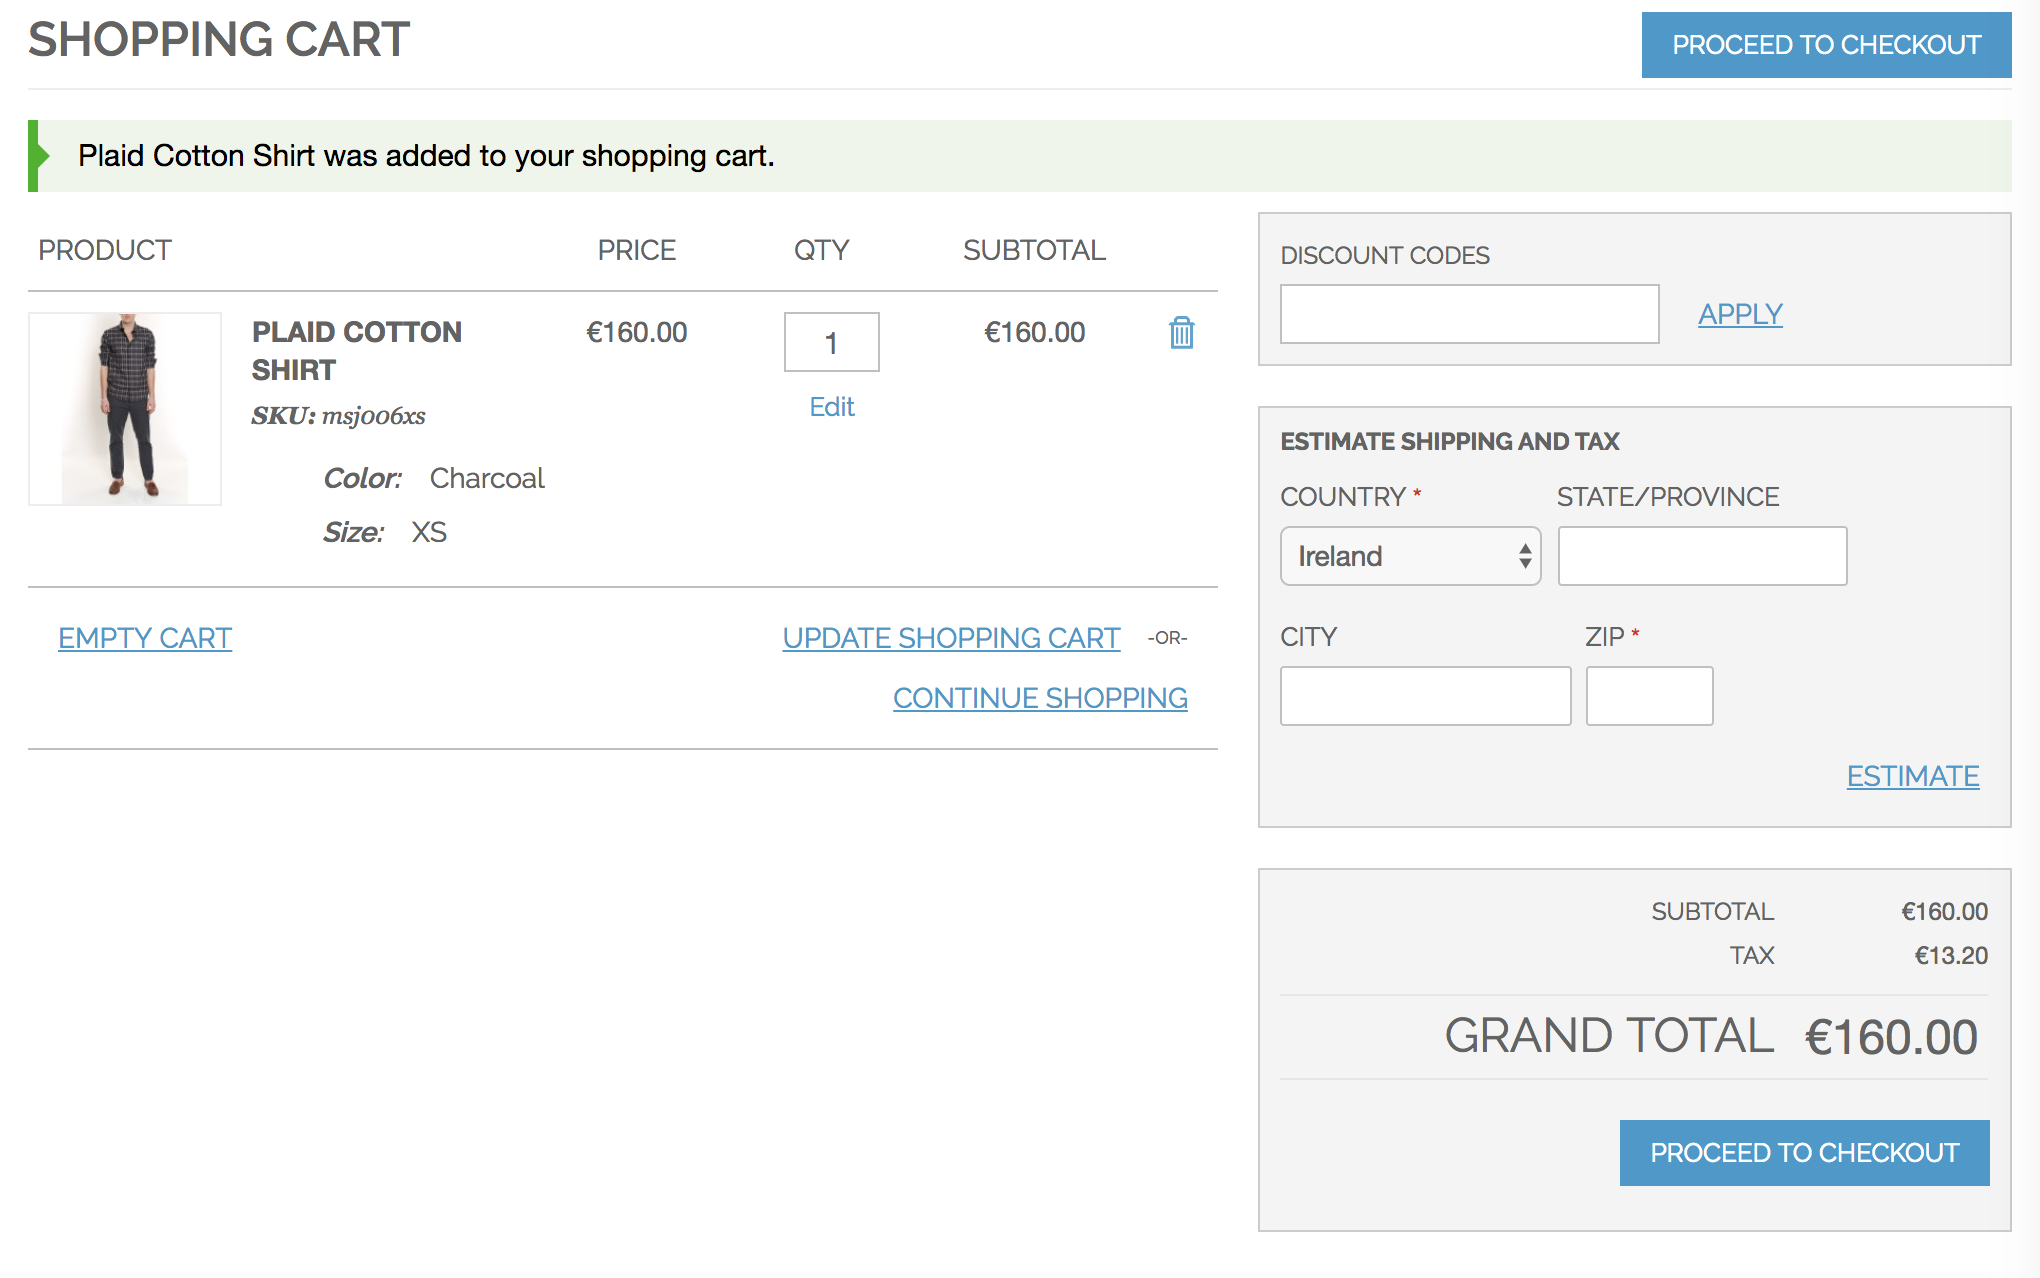
\includegraphics[height=10cm]{images/diagrams/before/desktop-shoppingcart.png}
  \caption{Shopping Cart Page Desktop Version}
  \label{fig:desktop-before-shoppingcart}
\end{figure}

\vspace{0.5cm}
\begin{figure}[H]
  \centering
    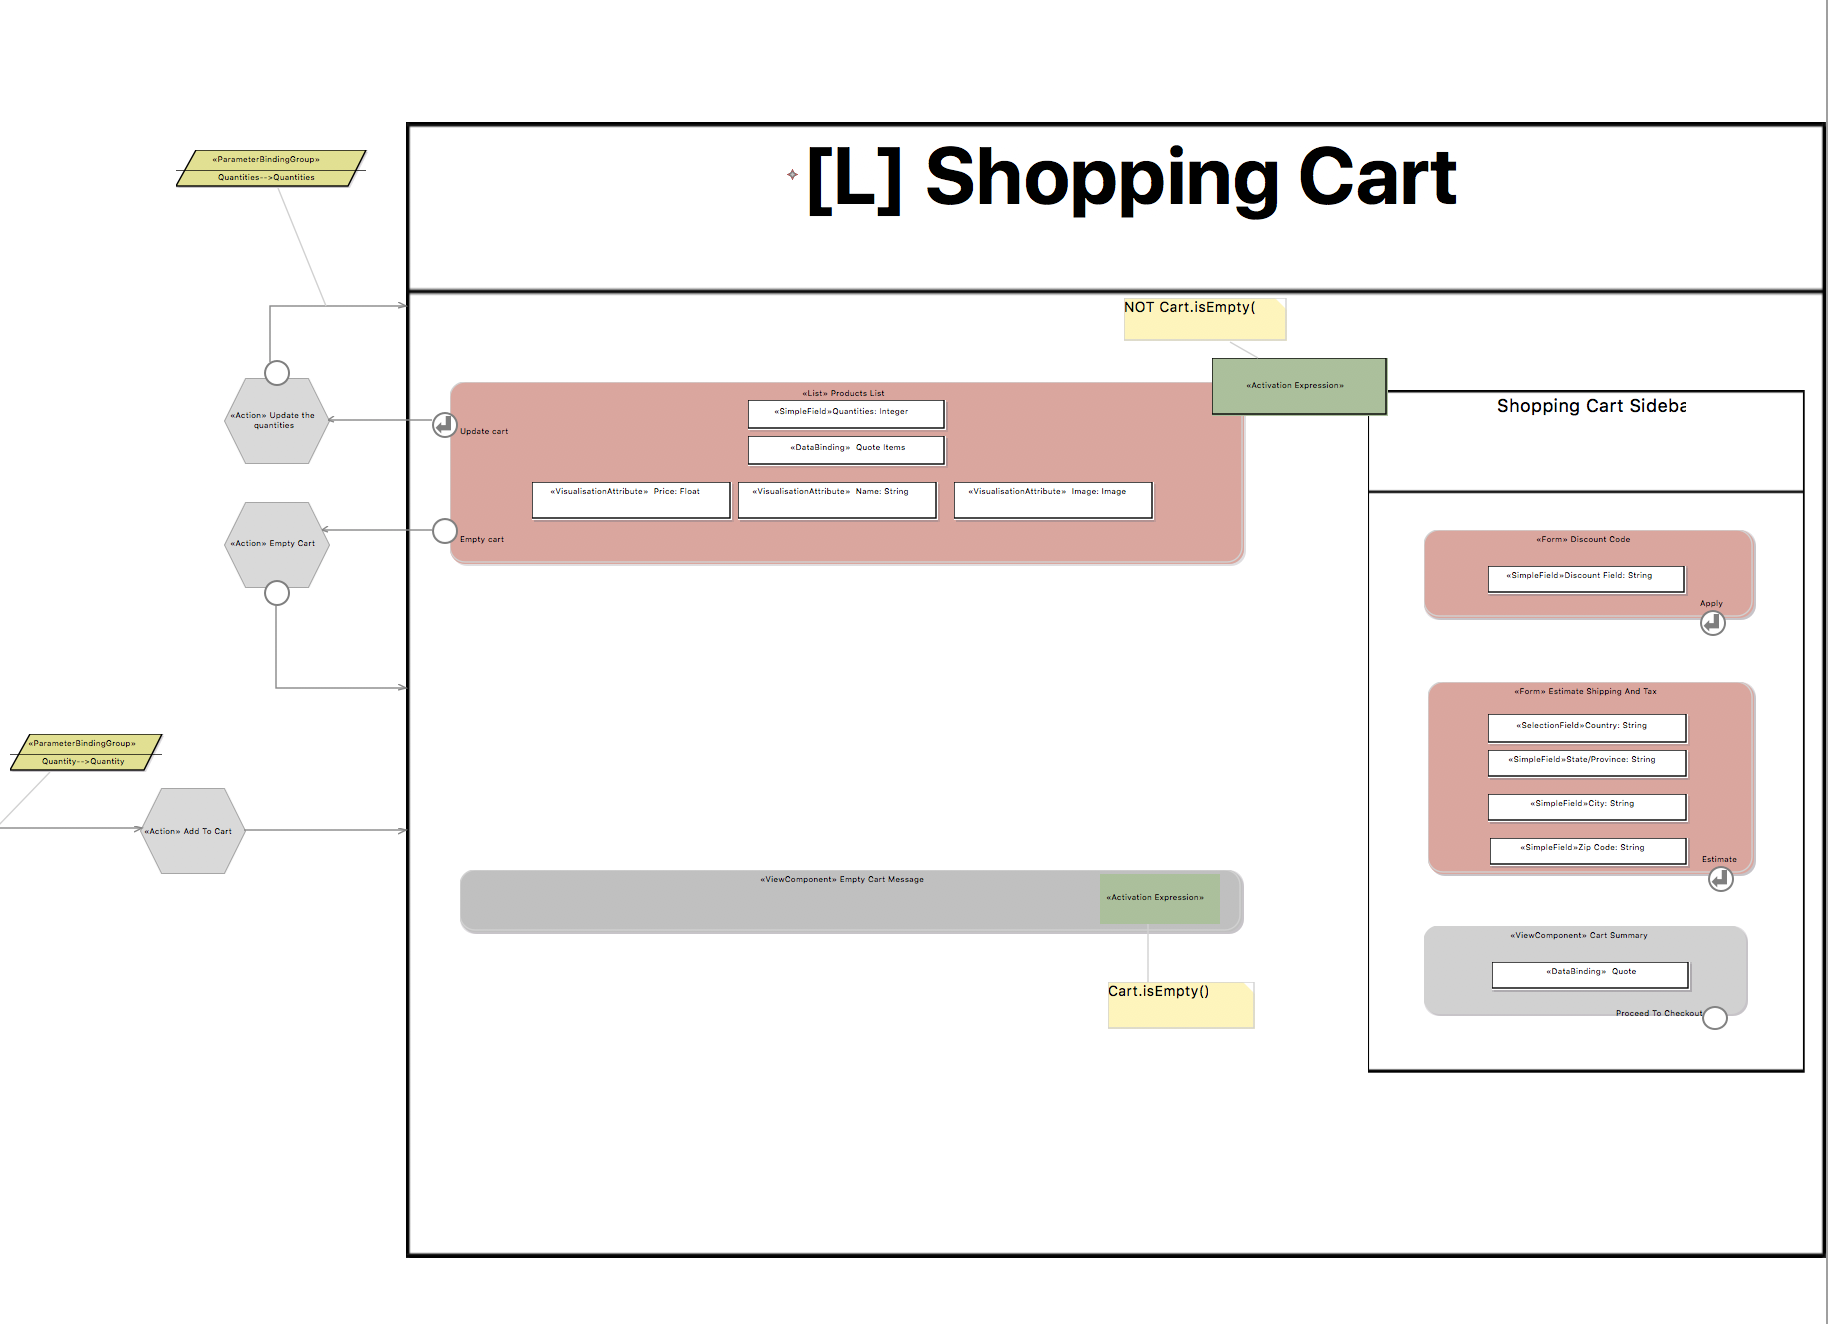
\includegraphics[height=10cm]{images/diagrams/before/ifml-shoppingcart.png}
  \caption{Shopping Cart Page IFML Diagram}
  \label{fig:ifml-before-shoppingcart}
\end{figure}
\vspace{0.5cm}

\newpage
As per shown in Figure \ref{fig:ifml-before-hierarchy-shoppingcart}, the Interaction Flow model representing the shopping page has the following form:

\lstset{language=XML}
\begin{lstlisting} 
    <interactionFlowModelElements xsi:type="ext:IFMLWindow"  name="Product" inInteractionFlows="//@interactionFlowModel/@interactionFlowModelElements.1/@viewElements.2/@viewElementEvents.0/@outInteractionFlows.0 //@interactionFlowModel/@interactionFlowModelElements.0/@viewElements.2/@viewElementEvents.0/@outInteractionFlows.0 //@interactionFlowModel/@interactionFlowModelElements.10/@viewElements.0/@viewElementEvents.0/@outInteractionFlows.0 //@interactionFlowModel/@interactionFlowModelElements.6/@viewElements.1/@viewElements.0/@viewElementEvents.0/@outInteractionFlows.0">
      <parameters  name="Product" />
      <viewElements xsi:type="ext:Details"  name="ProductDetails">
        <viewComponentParts xsi:type="core:DataBinding"  name="Product" uniformResourceIdentifier="">
          <subViewComponentParts xsi:type="core:VisualizationAttribute"  name="Price" featureConcept="//@domainModel/@domainElements.9"/>
          <subViewComponentParts xsi:type="core:VisualizationAttribute"  name="Image" featureConcept="//@domainModel/@domainElements.7"/>
          <subViewComponentParts xsi:type="core:VisualizationAttribute"  name="Name" featureConcept="//@domainModel/@domainElements.8"/>
          <subViewComponentParts xsi:type="core:VisualizationAttribute"  name="Description" featureConcept="//@domainModel/@domainElements.10"/>
        </viewComponentParts>
      </viewElements>
      <viewElements xsi:type="ext:Form"  name="AddToCartForm">
        <viewElementEvents xsi:type="ext:OnSubmitEvent"  name="Add To Cart" viewElement="//@interactionFlowModel/@interactionFlowModelElements.1/@viewElements.1">
          <outInteractionFlows xsi:type="core:NavigationFlow"  targetInteractionFlowElement="//@interactionFlowModel/@interactionFlowModelElements.9">
            <parameterBindingGroup >
              <parameterBindings  sourceParameter="//@interactionFlowModel/@interactionFlowModelElements.1/@viewElements.1/@viewComponentParts.2" targetParameter="//@interactionFlowModel/@interactionFlowModelElements.1/@viewElements.1/@viewComponentParts.2"/>
            </parameterBindingGroup>
          </outInteractionFlows>
        </viewElementEvents>
        <viewComponentParts xsi:type="ext:SelectionField"  name="Color" />
        <viewComponentParts xsi:type="ext:SelectionField"  name="Size" />
        <viewComponentParts xsi:type="ext:SimpleField"  name="Quantity" />
      </viewElements>
      <viewElements xsi:type="ext:List"  name="RelatedProductList">
        <viewElementEvents xsi:type="ext:OnSelectEvent"  name="Product Selected" viewElement="//@interactionFlowModel/@interactionFlowModelElements.1/@viewElements.2">
          <outInteractionFlows xsi:type="core:NavigationFlow"  targetInteractionFlowElement="//@interactionFlowModel/@interactionFlowModelElements.1">
            <parameterBindingGroup >
              <parameterBindings  sourceParameter="//@interactionFlowModel/@interactionFlowModelElements.0/@viewElements.2/@parameters.0" targetParameter="//@interactionFlowModel/@interactionFlowModelElements.1/@parameters.0"/>
            </parameterBindingGroup>
          </outInteractionFlows>
        </viewElementEvents>
        <viewComponentParts xsi:type="core:DataBinding"  name="Product"/>
        <viewComponentParts xsi:type="core:VisualizationAttribute"  name="Image" featureConcept="//@domainModel/@domainElements.7"/>
        <viewComponentParts xsi:type="core:VisualizationAttribute"  name="Name" featureConcept="//@domainModel/@domainElements.8"/>
        <viewComponentParts xsi:type="core:VisualizationAttribute"  name="Price" featureConcept="//@domainModel/@domainElements.9"/>
      </viewElements>
    </interactionFlowModelElements>
\end{lstlisting}

\newpage
The Model representation of the Shopping Cart page structure is shown in Figure \ref{fig:ifml-before-hierarchy-shoppingcart}

\vspace{0.5cm}
\begin{figure}[H]
  \centering
    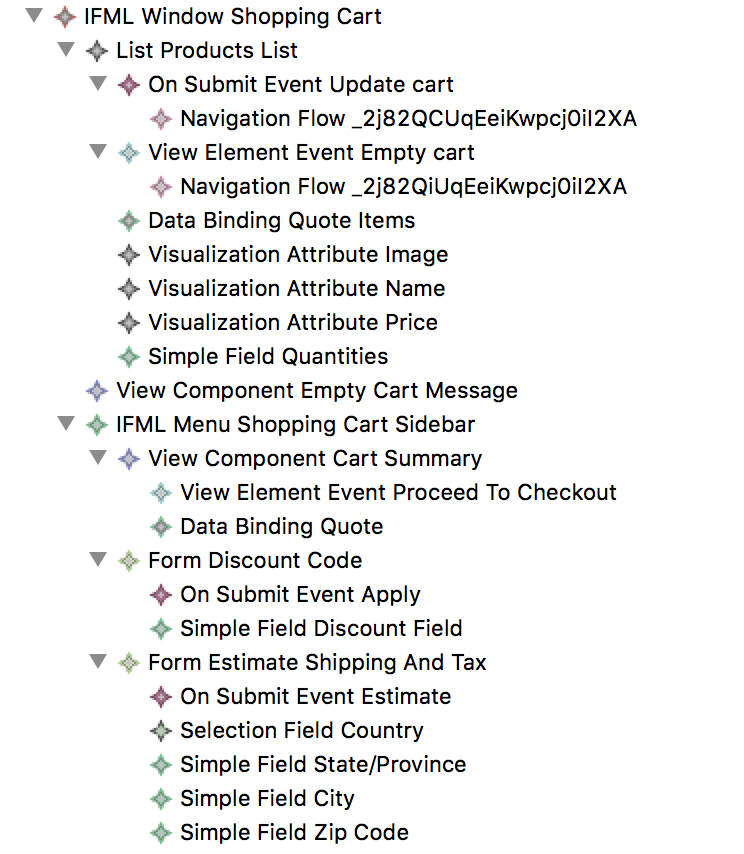
\includegraphics[height=10cm]{images/diagrams/before/ifml-hierarchy-shoppingcart.png}
  \caption{Interaction Flow Shopping Cart Model eCore representation}
  \label{fig:ifml-before-hierarchy-shoppingcart}
\end{figure}
\vspace{0.5cm}

\subsubsection{Shared Elements and Interactions}

As per previously mentioned, shared sections of the platform such as the Header and the Footer have been modeled as \textit{IFMLWindow} nodes reachable from any other area of the website, thus their \textit{Landmark} attribute set to true.
In more detail, the Header section contains a Navigation Menu in the form of a \textit{List View Component} with a children \textit{DataBinding} component correlated to the Category domain model and a simple \textit{Form View Component} for the search mechanism. When the user performs a search submitting a keyword the \textit{SearchKeyword} is triggered and the Search Keyword, based on the parameters held in the associated \textit{ParameterBinding} element, \textit{IFMLAction} is executed.  The resulting Search Results page, which presents a sidebar for filtering and a list of items matching the search, is another \textit{IFMLWindow} which structure resembles the "Product List Mode" for a Category Page described earlier (Figure \ref{fig:ifml-before-header-search}).

\vspace{0.5cm}
\begin{figure}[H]
  \centering
    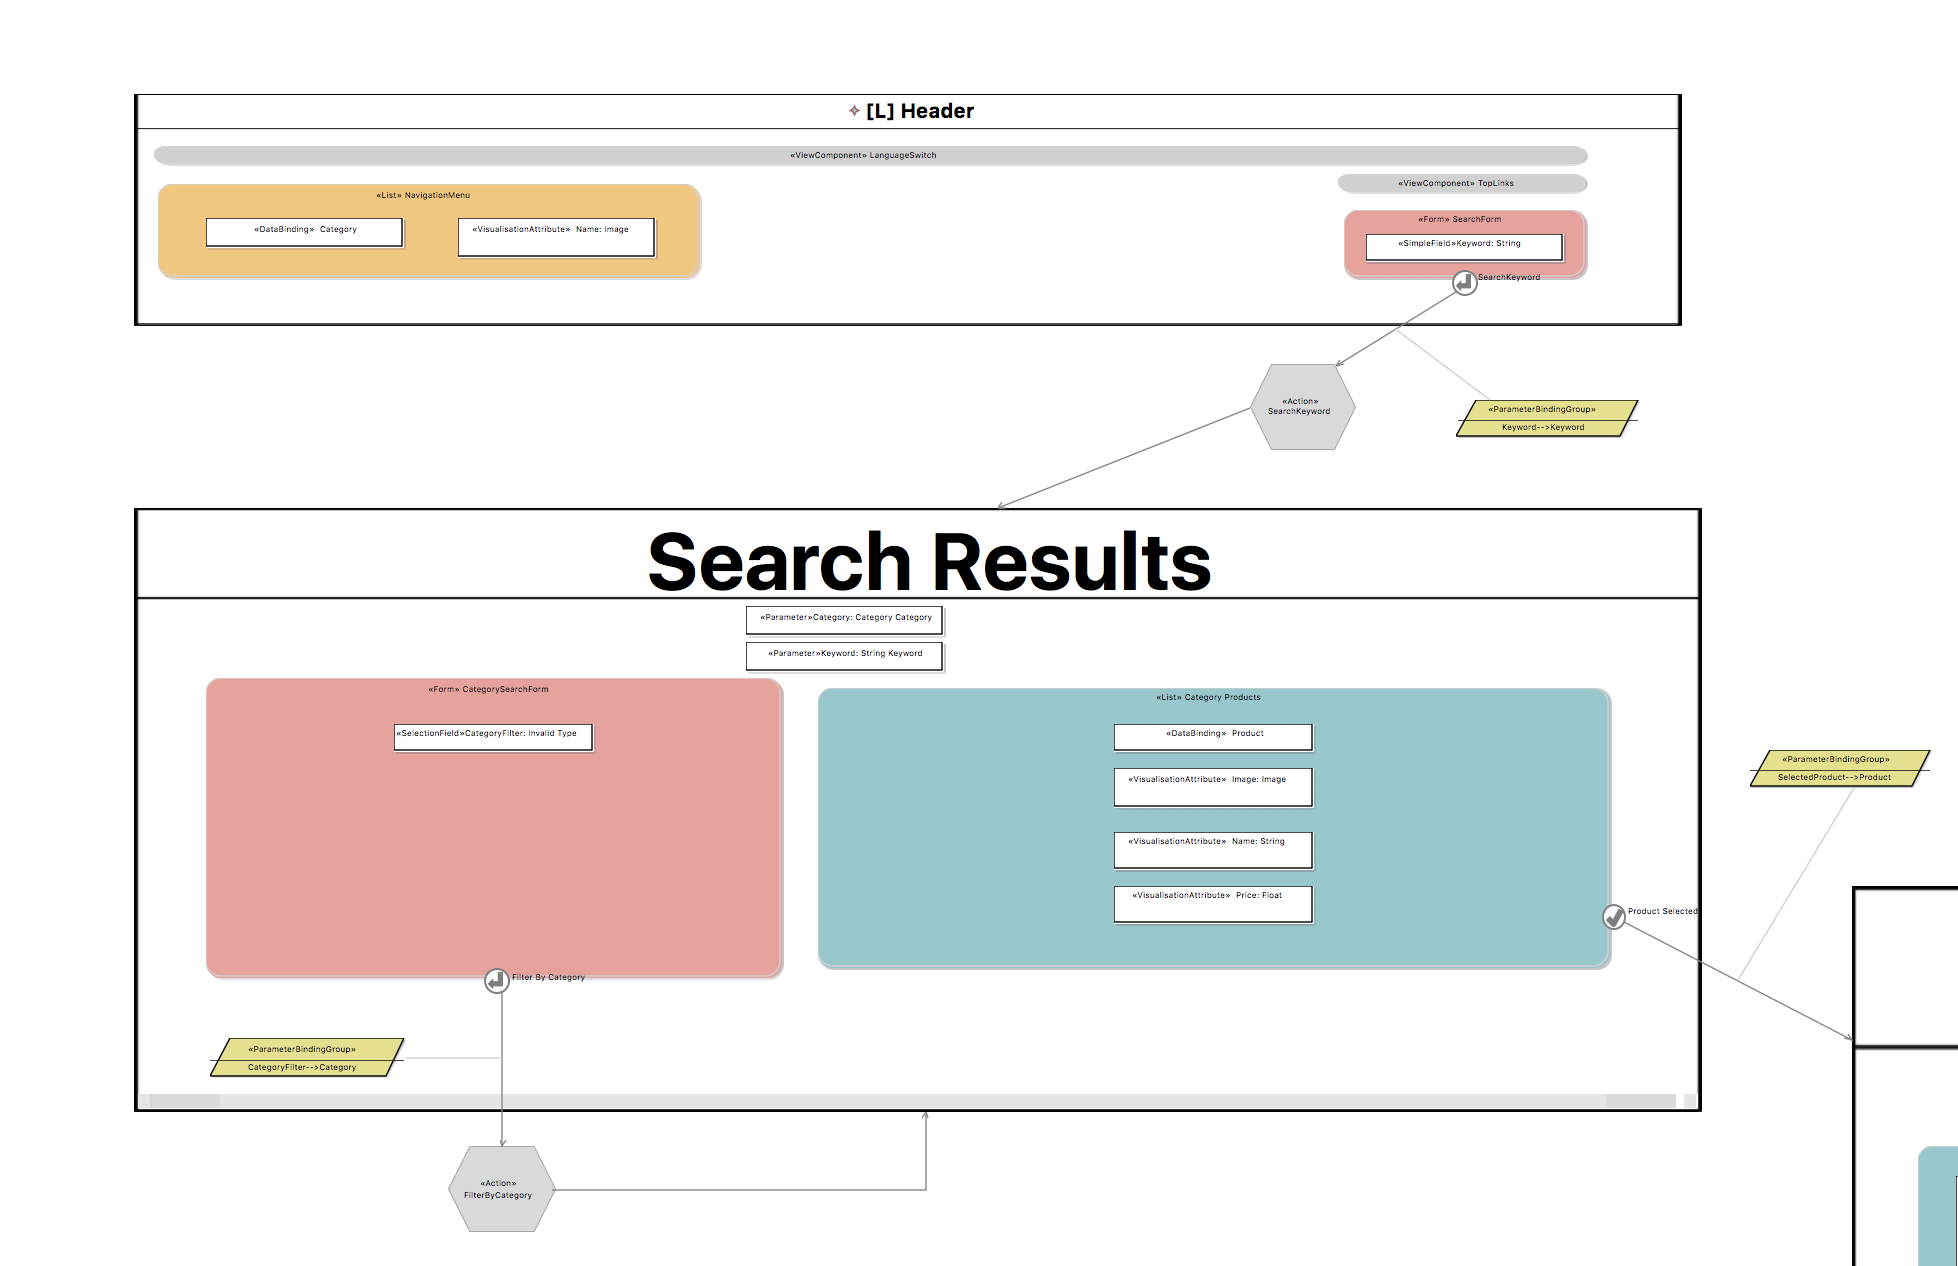
\includegraphics[height=10cm]{images/diagrams/before/ifml-header-search.png}
  \caption{Header and Search sections IFML Diagrams}
  \label{fig:ifml-before-header-search}
\end{figure}
\vspace{0.5cm}

The Footer \textit{IFMLWindow} model is quite straightforward, it retains the information about the footer links presented on the bottom of all the pages of the website in the form of a simple \textit{ViewComponent} and a Newsletter subscription \textit{Form View Component} reacting to SubscribeNewsletter submit \textit{Events}. Like for the header case we just described, the email passed as an argument from the \textit{Event} is carried to the \textit{IFMLAction} which, in this specific case, performs the actual Customer subscription and redirects to the current page.(Figure \ref{fig:ifml-before-footer}).

\vspace{0.5cm}
\begin{figure}[H]
  \centering
    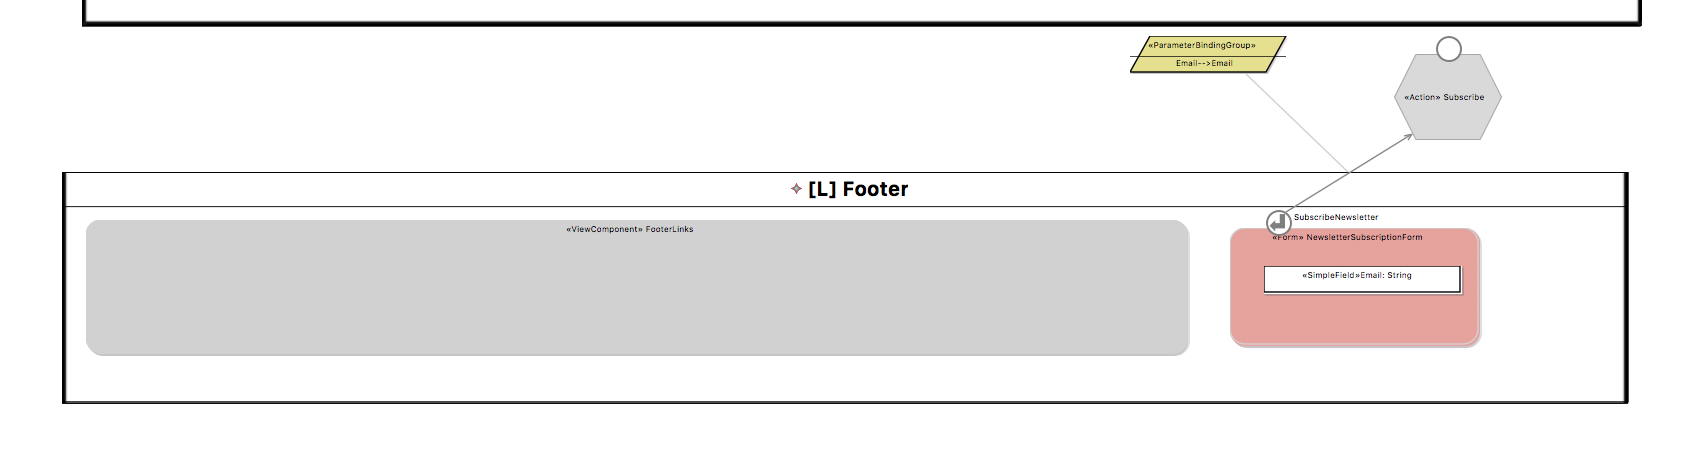
\includegraphics[width=12cm]{images/diagrams/before/ifml-footer.png}
  \caption{Footer section IFML Diagram}
  \label{fig:ifml-before-footer}
\end{figure}
\vspace{0.5cm}

We conclude this chapter with a snippet of the Header \textit{IFMLWindow} element code coming from the \textit{IFMLModel} and an excerpt of the eCore diagram for the areas of the website we described in this subsection (Figure \ref{fig:ifml-before-hierarchy-headersearchfooter}).

\lstset{language=XML}
\begin{lstlisting} 
  <interactionFlowModelElements xsi:type="ext:IFMLWindow" id="_LvuL0BPREei3TrqMA9Bdvw" name="Header" isLandmark="true">
  <viewElements xsi:type="ext:List" id="_v0p5YA9BEeiZ14TmPBeBNA" name="NavigationMenu">
    <viewComponentParts xsi:type="core:DataBinding" id="__mcXIA9BEeiZ14TmPBeBNA" name="Category"/>
    <viewComponentParts xsi:type="core:VisualizationAttribute" id="_Kbzt3xIZEeijSslFDgCgZA" name="Name" featureConcept="//@domainModel/@domainElements.5"/>
  </viewElements>
  <viewElements xsi:type="ext:Form" id="_YWvrMA9GEeiZ14TmPBeBNA" name="SearchForm">
    <viewElementEvents xsi:type="ext:OnSubmitEvent" id="_ULm7WRIWEeijSslFDgCgZA" name="SearchKeyword" viewElement="//@interactionFlowModel/@interactionFlowModelElements.4/@viewElements.1">
      <outInteractionFlows xsi:type="core:NavigationFlow" id="_Y6uV1xIWEeijSslFDgCgZA" targetInteractionFlowElement="//@interactionFlowModel/@interactionFlowModelElements.3">
        <parameterBindingGroup id="_yCY84hPOEei3TrqMA9Bdvw">
          <parameterBindings id="_y5vbohPOEei3TrqMA9Bdvw" sourceParameter="//@interactionFlowModel/@interactionFlowModelElements.4/@viewElements.1/@viewComponentParts.0" targetParameter="//@interactionFlowModel/@interactionFlowModelElements.3/@parameters.0"/>
        </parameterBindingGroup>
      </outInteractionFlows>
    </viewElementEvents>
    <viewComponentParts xsi:type="ext:SimpleField" id="_lWoCAA9GEeiZ14TmPBeBNA" name="Keyword" direction="out" />
  </viewElements>
  <viewElements xsi:type="core:ViewComponent" id="_aQFfjQ9TEeiZ14TmPBeBNA" name="TopLinks"/>
  <viewElements xsi:type="core:ViewComponent" id="_ezXdfQ9TEeiZ14TmPBeBNA" name="LanguageSwitch"/>
</interactionFlowModelElements>
\end{lstlisting}



\vspace{0.5cm}
\begin{figure}[H]
  \centering
    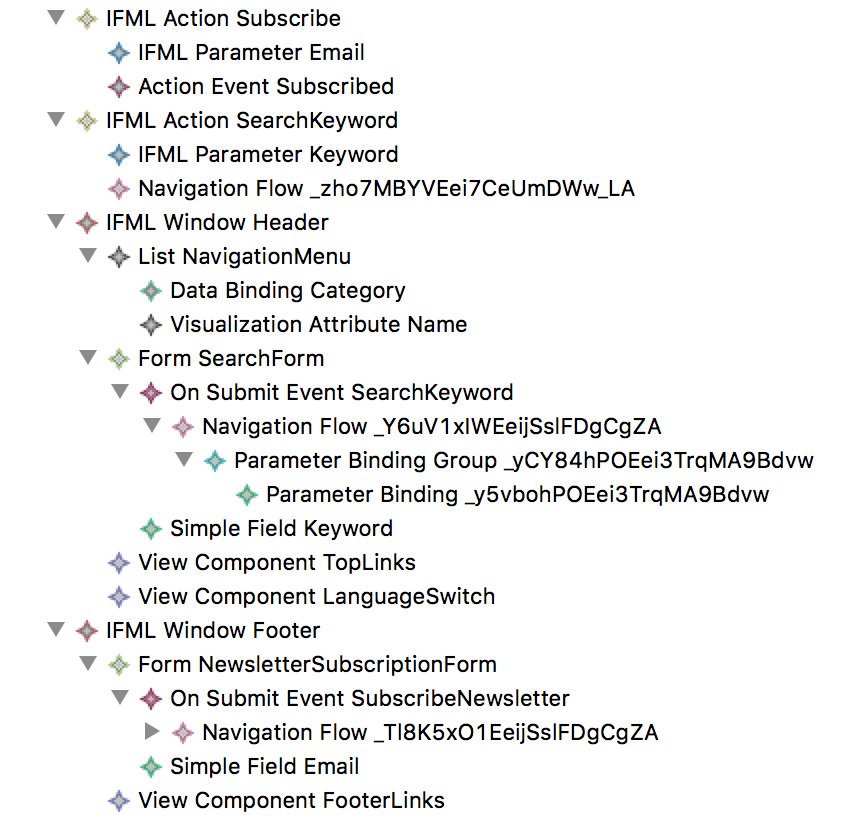
\includegraphics[height=10cm]{images/diagrams/before/ifml-hierarchy-headersearchfooter.png}
  \caption{Interaction Flow eCore representation for the shared elements}
  \label{fig:ifml-before-hierarchy-headersearchfooter}
\end{figure}
\vspace{0.5cm}
